\documentclass[a4paper, 12pt]{report}
\usepackage[a4paper,hmargin={3cm,2.5cm},vmargin={2.5cm,2.5cm}]{geometry}
\usepackage{amsfonts} % if you want blackboard bold symbols e.g. for real numbers
\usepackage{graphicx} % if you want to include jpeg or pdf pictures
\usepackage{multicol}
\usepackage{lipsum}
\usepackage{subfig}
\usepackage{float}
\usepackage{blindtext}
\usepackage{fancyhdr}
\pagestyle{fancy}
\lhead{}
\rhead{Bajaj Institute of Technology, Wardha}
\lfoot{Department of Computer Engineering}
\usepackage{tikz}
\usetikzlibrary{calc}
%\usepackage{eso-pic}
\usepackage{lipsum}
\usepackage{longtable}
\renewcommand{\bibname}{References}
\begin{document}
%========================================================= %
%================begin of title page====================== %
% The frontmatter environment for everything that comes with roman numbering\
%============================================= %
\newenvironment{frontmatter}{}{}
\begin{frontmatter}
%%%%%%%%%%%%%%%%%%%%%%%%%%%%%%%%%%%%%%%%%%%%%%%%%%%%%%%%%%%%%%%%%%%
\begin{titlepage}
%\AddToShipoutPictureBG
\begin{center}	
	\begin{LARGE}
		{\textbf {Sentimental Analysis for Hotel Review}}
	\end{LARGE}\\[0.5cm]
	
	\textit{\textbf{A project report submitted to}}\\
	\textit{\textbf{Dr. Babasaheb Ambedkar Technological University, Lonere}}\\
	\textit{\textbf{in partial fulfillment of the requirements for the award of the degree}}\\[0.5cm]
	\textup{\large \textbf{Bachelor of Technology}\\[0.1cm]
		in\\[0.1cm]
		\textbf{Computer Engineering}}\\[0.2cm]	
		\vspace{0.5cm}
		\textbf{\large Mini-Project – I}\\[0.25cm]\textbf{\small (BTCOM507)}

	\begin{center}
		\begin{figure}[h]  %h means here other options t , b, p, etc.
		\centering
		
\includegraphics[width=0.25\linewidth]{./logo1}
		\end{figure}
	\end{center}

	\textit{by}\\[0.3cm]
	\textbf{Mr. Prajwal Rameshwar Gurnule (PRN: 2146491245011)}\\[0.25cm]
	\textbf{Mr. Pranav Vijay Ikhar (PRN: 2146491245009)}\\[0.25cm]
	\textbf{Miss Renuka Ashok Kothekar (PRN: 2146491245016)}\\[0.25cm]
	\textbf{Miss Ritika Vinayakrao Bhonge (PRN: 2146491245003)}\\[0.25cm]
	(V Semester)
	\\[0.5cm]	
	
	\textit{under the guidance of}\\[0.25cm]
	\textbf{Mr. Amol Jumde}\\[0.25cm]	
	(Assistant Professor)\\[0.5cm]
	\vspace{0.2cm}
	
	\textup{\textbf{\large Department of Computer Engineering}\\[0.1cm]
		Shiksha Mandal's\\
		[0.1cm]
		\textbf{BAJAJ INSTITUTE OF TECHNOLOGY, WARDHA}}\\[0.1cm]Pipri, Arvi Road, Wardha - 442001.\\[0.2cm]
	
	\textbf{(2023-24)}
\end{center}
\end{titlepage}
%================end of title page======================

%================begin of certificate page======================
\begin{titlepage}
\begin{tikzpicture}[overlay,remember picture]
\draw[line width=4pt]
    ($ (current page.north west) + (1cm,-1cm) $)
    rectangle
    ($ (current page.south east) + (-1cm,1cm) $);
\draw[line width=1.5pt]
    ($ (current page.north west) + (1.2cm,-1.2cm) $)
    rectangle
    ($ (current page.south east) + (-1.2cm,1.2cm) $);
\end{tikzpicture}
\begin{center}
	\textup{\large  \textbf{Dr. Babasaheb Ambedkar Technological University, Lonere}\\
	\textbf{Bajaj Institute of Technology, Wardha}}\\
	Pipri, Arvi Road, Wardha - 442001.\\[0.5cm]
	\textbf{\large DEPARTMENT OF COMPUTER ENGINEERING}
	
	%---------------------------------Figure-----------------
	\begin{figure}[h]
	\centering
	
\includegraphics[width=0.3\linewidth]{./logo1}
	\end{figure}	
	%-------------------------------------------------------
	\begin{LARGE}
	\textbf{\textit {Certificate}}
	\end{LARGE}\\[1.2cm]
	This is to certify that Mini-Project-I titled\\[0.5cm]
	\begin{large}
	\large\textbf{Sentimental Analysis for Hotel Review}
	\end{large}\\[0.8cm] 
	
	has been completed by \\[0.8cm]
	\textbf{Mr. Prajwal Rameshwar Gurnule (PRN: 2146491245011)}\\[0.25cm]
	\textbf{Mr. Pranav Vijay Ikhar (PRN: 2146491245009)}\\[0.25cm]
	\textbf{Miss Renuka Ashok Kothekar (PRN: 2146491245016)}\\[0.25cm]
	\textbf{Miss Ritika Vinayakrao Bhonge (PRN: 2146491245003)}\\[0.25cm]
\end{center}
of V Semester (Sec: A), Computer Engineering of academic year 2023-24 in partial fulfillment of Mini-Project-I (BTCOM507) course as prescribed by the Dr. Babasaheb Ambedkar Technological University, Lonere.
\vspace{1.5cm}

\begin{multicols}{2}
\begin{center}
\textbf{Amol Jumde}\hspace{5cm}\\
(Project Guide)\hspace{5cm}\\
\end{center}

\begin{center}
\textbf{Prof. Sheetal Kale}\\
(Head of the Department)\\
\end{center}
\vspace{1.0cm}
\end{multicols}

\hbox {Place: BIT, Wardha\\}
\hbox {Date: \today\\}
\end{titlepage}
%================end of certificate page======================


\thispagestyle{empty}
\begin{center}
\begin{LARGE}
	\textbf{\textit {Declaration}}\end{LARGE}\\[1.2cm]
\end{center}
I hereby declare that the Mini Project report titled \textbf{``Sentimental Analysis for   Hotel Review"} submitted by me to the Bajaj Institute of Technology, Wardha, in partial fulfilment of the requirement for the award of Degree of B. Tech in Computer Engineering is a record of bonafide seminar work carried out by me under the guidance of Mr. Amol Jumde.\\

I, further declare that the work reported in this Mini Project report has not been submitted either in-part or in-full for the award of any other degree in any other Institute or University.\\

{\flushleft\textbf{Report Title}: Sentimental Analysis for Hotel Review}\\
\begin{table}[h]
	\begin{tabular}{|p{1cm}|p{5cm}|p{3cm}|p{4cm}|}
		\hline
		\textbf{SN} & \textbf{Student Name} & \textbf{PRN} & \textbf{Signature} \\
		\hline
		1 &Prajwal Gurnule &2146491245011 & \\
		\hline
		2 &Pranav Ikhar &2146491245009 & \\
		\hline
		3 &Renuka Kothekar &2146491245016 & \\
		\hline
		4 &Ritika Bhonge &2146491245003 & \\
		\hline
	\end{tabular}
\end{table}

{\flushleft
\textbf{Date}: \today\\
\textbf{Place}: BIT, Wardha  
}
\newpage
\thispagestyle{empty}
\begin{center}
	\begin{LARGE}
		\textbf{\textit {Acknowledgment}}\end{LARGE}\\[1.2cm]
\end{center}
I would like to express my gratitude and appreciation to all those who gave me the
possibility to complete this report. Special thanks is due to my Guide Mr. Amol Jumde, Assistant Professor of Computer Engineering whose help, stimulating suggestions and encouragement helped me in all
time of process and in writing this report. I extend my heartfelt thanks to Prof. Sheetal Kale, Head of the Department Computer Engineering Bajaj Institute of Technology, Wardha for her insightful guidance, assistance and invaluable suggestions that significantly enriched the quality of these work.  I also sincerely thanks for the time spent proofreading and correcting my many mistakes. My deepest thanks to Department of Computer Engineering And Dr. Narendra Kanhe,
Principal Bajaj of Institute of Technology, Wardha. I would also like to acknowledge
with much appreciation the crucial role of the staff in Computer Lab, who gave me a
permission to use the Computers in the laboratory. Many thanks go to the all lecturers
and go to all my classmates, especially to my friends for spending their time in helping
and giving support whenever I need it in My Mini Project Topic.
\\


%%%%%%%%%%%%%%% Abstract %%%%%%%%%%
\newpage
\thispagestyle{empty}
\begin{center}
	\begin{LARGE}
		\textbf{\textit {Abstract}}\end{LARGE}\\[1.2cm]
\end{center}

Hotel review analysis is a process of analyzing customer feedback on hotels to extract useful insights and 
patterns. This analysis can be done through various techniques such as sentiment analysis, topic modeling, and 
natural language processing. The abstract of a hotel review analysis would summarize the key findings and 
insights obtained from the analysis. This could include information on the most common positive and negative 
aspects of the hotel, the most commonly mentioned amenities, and the sentiment of customer feedback. The 
abstract may also highlight any notable trends or patterns in the data, such as changes in customer sentiment 
over time or differences in feedback across different demographics. A hotel review analysis abstract would 
provide a concise and informative summary of the key takeaways from the analysis, helping stakeholders to 
understand customer feedback and make data-driven decisions to improve their hotel offerings.
\\

In this project, sentiment analysis is performed on the basis of user reviews using five different
classifiers. The classifiers used in this project are K Neighbours Classifier , 
Decision Tree Classifier , Random Forest Classifier , Support Vector Machine (SVM) , Multinomial Naive Bayes , Multilayer Perceptron Classifier. The performance of these algorithms are assessed on two different parameter
settings. The reviews are classified as “positive”,“negative” or “average” labels.
	\vspace{0.3cm}
	
	\textbf{Keywords- }\textbf{\textit{Sentimental Analysis}, \textit{Classification}, \textit{Machine learning}, \textit{Opinion mining}}

%================================================ %

\newpage
\thispagestyle{empty}
\begin{center}
	\begin{LARGE}
		\textbf{\textit {Abbreviations}}\end{LARGE}\\[1.2cm]
\end{center}

\begin{table}[h]
	\begin{tabular}{ll}			
		\textit{SVM} & Support Vector Machine \\
		\textit{MLP} & Multilayer Perceptron \\	
		\textit{NLP} & Natural Language Processing \\	
		\textit{NLTK} & Natural Language Toolkit \\	
		\textit{API} & Application Programming Interface \\	
	\end{tabular}
\end{table}
%================================================ %

\pagenumbering{gobble}
\pagebreak
\pagenumbering{roman}
\setcounter{page}{1}
\newpage
\tableofcontents
\listoffigures
% \lfoot{Bajaj Institute of Technology, Wardha}
\newpage


% The frontmatter environment for everything that comes with roman numbering %
\end{frontmatter}
%%%%%%%%%%%%%%%%%%%%%%%%%%%%%%%%%%%%%%%

\newpage
\pagenumbering{arabic}
%%%%%%%%% MAIN TEXT STARTS HERE %%%%%%%%%%
\chapter{Introduction}
\par The growing popularity of online booking platforms, hotel reviews have become a valuable source of 
information for travellers when making their accommodation choices. However, analysing the vast amount of 
text data contained in these reviews manually is a time-consuming and labour-intensive task. Hence, there is a 
need to develop automated methods for sentiment analysis of hotel reviews. Sentiment analysis, also known as 
opinion mining, is the process of automatically identifying and classifying subjective information from text data. 
It involves analyzing the language and tone used in text to determine whether it expresses positive, negative, or 
neutral sentiment. Sentiment analysis has a wide range of applications in industries such as marketing, 
customer service, and product development, where understanding customer opinions and feedback is crucial.
\\
\par In this project, we aim to develop a machine learning model that can perform sentiment analysis on hotel 
reviews to determine the overall sentiment expressed in the review. The model will be trained using a dataset 
of hotel reviews that have been labelled with their corresponding sentiment. The dataset will be pre-processed 
to remove irrelevant information, such as stop words and punctuation, and transformed into numerical 
features that can be used as input to the machine learning model.
We will explore a variety of machine learning algorithms, including Naive Bayes, Logistic Regression, Support 
Vector Machines (SVM), and Random Forests, to identify the most effective algorithm for sentiment analysis of 
hotel reviews. We will evaluate the performance of each algorithm using standard evaluation metrics such as 
accuracy, precision, recall, and F1-score.
The proposed project has practical applications in the hospitality industry, where it can be used to 
automatically analyse customer feedback and identify areas for improvement in hotel services.
\\ 
\par The project can 
also be extended to other domains such as e-commerce, social media, and healthcare, where sentiment analysis 
can provide valuable insights into customer behaviour and preferences.
\section{Motivation}

Sentiment analysis of hotel reviews can provide valuable insights into customer satisfaction and identify areas where a hotel can improve. By understanding the overall sentiment of hotel reviews, hoteliers can gain a better understanding of the customer experience and make data-driven decisions to improve their services and attract more guests.\\
Motivations for conducting sentiment analysis of hotel reviews:\\
\textbf{Identify customer satisfaction levels:}Sentiment analysis can be used to determine whether the overall sentiment of hotel reviews is positive, negative, or neutral. This can give hoteliers a general sense of how satisfied their guests are with their hotel stay.\\
\textbf{Understand customer feedback:} Sentiment analysis can also be used to identify specific aspects of the hotel experience that customers are satisfied or dissatisfied with. This can help hoteliers to pinpoint areas where they can improve their services.\\
\textbf{Track sentiment over time:}
Track sentiment over time: Sentiment analysis can be used to track the sentiment of hotel reviews over time. This can help hoteliers to identify trends in customer satisfaction and see how their efforts to improve their services are impacting guest feedback.\\
\textbf{Benchmark against competitors:} Sentiment analysis can be used to compare the sentiment of hotel reviews to the sentiment of reviews of competitor hotels. This can help hoteliers to identify areas where they are excelling and areas where they can improve their competitive standing.
\section{Background}
\textbf{Benefits of Sentiment Analysis for Hotel Reviews}\\
There are a number of benefits to using sentiment analysis for hotel reviews.\\
These benefits include:\\
\textbf{Improved customer satisfaction:} By understanding the sentiment of their guests, hoteliers can make data-driven decisions to improve their services and attract more guests.\\
\textbf{Identification of areas for improvement:} Sentiment analysis can help hoteliers to identify specific areas where they can improve their services. This can include things like upgrading amenities, improving staff training, or changing policies.\\
\textbf{Tracking sentiment over time:} Sentiment analysis can be used to track the sentiment of hotel reviews over time. This can help hoteliers to identify trends in customer satisfaction.\\
\textbf{Benchmarking against competitors:} Sentiment analysis can be used to compare the sentiment of hotel reviews to the sentiment of reviews of competitor hotels. This can help hoteliers to identify areas where they are excelling and areas where they can improve their competitive standing.
\\
\\
\textbf{Challenges of Sentiment Analysis for Hotel Reviews}\\
There are a number of challenges to using sentiment analysis for hotel reviews. These challenges include:\\
\textbf{Sarcasm and irony:} It can be difficult for sentiment analysis tools to detect sarcasm and irony, which can lead to inaccurate sentiment classifications.\\
\textbf{Subjectivity:} Sentiment analysis is based on the subjective opinions of reviewers, which can lead to varying interpretations of the same review.\\
\textbf{Lack of contextual information:} Sentiment analysis tools often do not have access to contextual information about the hotel stay, such as the time of year or the purpose of the trip. This can make it difficult for them to accurately assess the sentiment of the review.
\section{Problem statement}
Determine the sentiment (positive, negative, or neutral) of hotel reviews based on the text provided in the reviews. The goal is to classify these reviews accurately to help hotels assess customer satisfaction and improve their services.
\\
This problem statement sets the objective of analyzing hotel reviews, which can be used in various applications, including improving customer experiences and enhancing hotel services.
\\
The purpose of sentiment analysis of hotel reviews is to understand the overall sentiment of guests towards a hotel, its services, and its amenities. This information can be used by hotels to improve their guest experience, identify areas for improvement, and make better business decisions.\\
In sentiment analysis of hotel reviews can help hotels to:
\begin{itemize}
	\item Understand what guests like and dislike about their hotel
	\item Identify areas where they can improve the guest experience
	\item Make better business decisions, such as how to price their rooms and what amenities to offer
\end{itemize}
Sentiment analysis is a valuable tool for hotels that want to stay ahead of the competition and provide their guests with the best possible experience.
\section{Objectives}
\par The main objectives of the projects are as follows:
\begin{itemize}
	\item  \textbf{Understanding Customer Sentiments:} Sentiment analysis helps in comprehending the sentiments expressed by hotel guests in their reviews. It allows businesses to gauge customer satisfaction or dissatisfaction with their services and facilities. 
	\item  \textbf{Designing Machine Learning Tools:} Researchers and data scientists design machine learning models and algorithms to automate sentiment analysis of hotel reviews. These models can be fine-tuned to extract sentiments accurately from textual data 
	\item  \textbf{Analyzing Customer Feedback:} Sentiment analysis enables in-depth analysis of customer feedback. It categorizes reviews as positive, negative, or neutral, helping hotels identify specific areas that require improvement 
	\item  \textbf{Creating Data-Driven Insights:} The process of sentiment analysis creates valuable data-driven insights. These insights can inform hotel management about the strengths and weaknesses of their operations, guiding strategic decisions 
	\item  \textbf{Implementing Improvements:} By implementing the findings from sentiment analysis, hotels can make necessary improvements to enhance customer satisfaction. This could include changes in services, facilities, or staff training. 
\end{itemize}

\section{Sentimental Analysis Work Flow}
The image shown in Figure 1.1 , a block diagram of a Sentiment Analysis Experimental Workflow. The system is designed to train and validate a model that can predict the sentiment of text reviews, such as whether they are positive or negative. The system uses a variety of data preprocessing and feature engineering techniques to prepare the data for training, including text preprocessing, train-test split, and TF-IDF vectorization. The model is trained using a random undersampling technique to address the imbalance between positive and negative reviews. The trained model is then evaluated on a held-out test set to assess its performance.
\begin{figure}[h]
	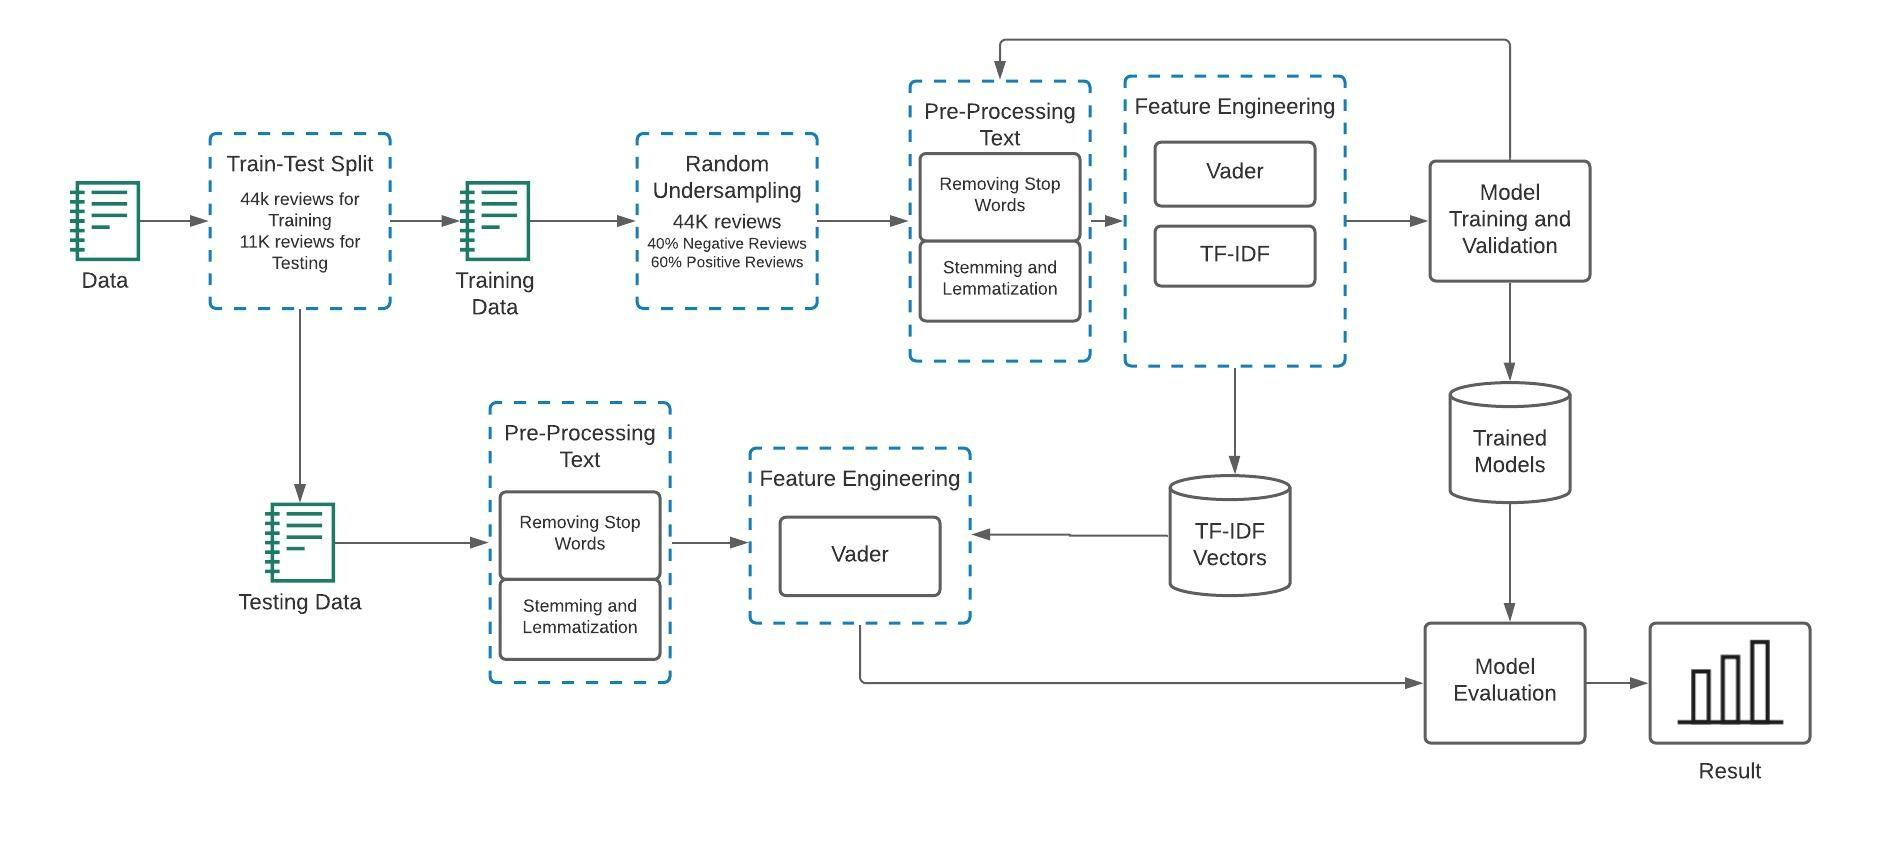
\includegraphics[height=3.5in,width=6in]{c}
	\caption{Sentiment Analysis Experimental Workflow }
	\label{Fig.}
\end{figure}\\
\textbf{Preprocessing:}
The preprocessing step is important to ensure that the data is in a format that can be easily understood by the sentiment analysis model. This may involve:
\begin{itemize}
	\item \textbf{Cleaning the data:} This may involve removing punctuation, correcting spelling errors, and converting all text to lowercase.
	\item \textbf{Removing stop words:} Stop words are common words that do not add much meaning to a sentence, such as "the", "is", and "and". Removing stop words can help to improve the performance of the sentiment analysis model.
	\item \textbf{Stemming and lemmatizing:} Stemming and lemmatizing are techniques that reduce words to their root form. This can help to improve the performance of the sentiment analysis model by reducing the number of unique words that it needs to learn.
\end{itemize}
\textbf{Feature engineering:}
The feature engineering step involves extracting features from the data that will help the sentiment analysis model to make accurate predictions. Common features include:
\begin{itemize}
	\item \textbf{The word count:} The number of words in a sentence can be used as a feature to indicate the length and complexity of the sentence.
	\item \textbf{The number of positive and negative words:} The number of positive and negative words in a sentence can be used to indicate the overall sentiment of the sentence.
	\item \textbf{The presence of certain keywords or phrases:} The presence of certain keywords or phrases in a sentence can be used to indicate the topic of the sentence and the sentiment of the author towards that topic.
\end{itemize}
\textbf{Model training:}
The model training step involves training a sentiment analysis model on the preprocessed data. There are a variety of different machine learning algorithms that can be used for sentiment analysis, such as Naive Bayes, Support Vector Machines, and Long Short-Term Memory (LSTM) networks.\\
The choice of algorithm will depend on the specific problem that you are trying to solve and the amount of data that you have available. For example, Naive Bayes is a simple algorithm that is easy to train and interpret, but it may not be as accurate as more complex algorithms, such as LSTM networks.
\\
\textbf{Model evaluation:} Once sentiment analysis model have trained, We need to evaluate its performance on a held-out test set. This will give us an idea of how well the model will generalize to new data.\\
To evaluate the model, you can use a variety of metrics, such as accuracy, precision, recall, and F1 score. Accuracy is the percentage of predictions that the model makes correctly. Precision is the percentage of positive predictions that are actually correct. Recall is the percentage of all positive examples that are correctly identified by the model. F1 score is a harmonic mean of precision and recall.
\\
\textbf{Model deployment:} Once sentiment analysis model are satisfied with the performance , then deploy it to production. This may involve integrating the model into a web application.\\
Once the model is deployed, you can use it to analyze new data and generate sentiment insights. For example, we use the model to analyze customer reviews to identify areas where our product or service can be improved.
\chapter{Literature Survey}
\section{Literature review}
\underline{\textbf{1. A Sentiment-Based Hotel Review Summarization}}\\
\textbf{o	Year of Publication} - 2017\\
\textbf{o	Author} - Hegde, Y., and S. Padma \\
\textbf{o	Objective} - An overview of a review management tool is shown where a variety of hotel comments were collected, in order to hark the visitors’ points and views of the hotel quality.\\ 
\textbf{o   Abstraction} - We can found some basic reviews in user review and also can find user own opinions about the experience with various products. Many users read the reviews of the information given on the Web to take decisions such as buying products, watching movie, going to restaurant, etc. It is difficult for Web users to read and understand the contents from a large number of reviews. The important and useful information can be extracted from the reviews through opinion mining and summarization process. We obtained about 78.2 percent of accuracy of hotel review classification as positive or negative review by machine learning method. The classified and summarized hotel review information helps the Web users to understand the review contents easily in a short time.\\ 
\textbf{o	Conclusion} - The classified and summarized hotel review information helps the Web users to understand the review contents easily in a short time. 
\\
\\
\underline{\textbf{2. A comparative assessment of star ratings for consumer reviews}}\\
\textbf{o	Year of Publication} - 2020\\
\textbf{o	Author} - Sameh Al-Natour, Ozgur Turetken \\
\textbf{o	Objective} - It is crucial to optimize the Naive Bayes technique because its level of accuracy still has flaws. In 
order to achieve a higher level of accuracy, optimization employs the right and best techniques for text 
grouping, particularly for hotel review classification.\\ 
\textbf{o   Abstraction} - In this paper, we explore the viability of automatic sentiment analysis (SA) for assessing the polarity of a product or a service review. To do so, we examine the potential of the major approaches to sentiment analysis, along with star ratings, in capturing the true sentiment of a review. We further model contextual factors (specifically, product type and review length) as two moderators affecting SA accuracy. The results of our analysis of 900 reviews suggest that different tools representing the main approaches to SA display differing levels of accuracy, yet overall, SA is very effective in detecting the underlying tone of the analyzed content, and can be used as a complement or an alternative to star ratings.\\ 
\textbf{o	Conclusion} - The results further reveal that contextual factors such as product type and review length, play a role in affecting the ability of a technique to reflect the true sentiment of a review. 
\\
\\
\underline{\textbf{3. Sentiment Analysis for Hotel Reviews}}\\
\textbf{o	Year of Publication} - 2017\\
\textbf{o	Author} - Walter Kasper, Mihaela Vela\\
\textbf{o	Objective} - An overview of a review management tool is shown where a variety
of hotel comments were collected, in order to hark the visitors’ points and views
of the hotel quality\\ 
\textbf{o   Abstraction} - User reviews and comments on hotels on the web are  an important information source in travel planning. Therefore,  knowing about these comments is important for quality control  to the hotel management, too. We present a system that collects  such comments from the web and creates classified and structured overviews of such comments and facilitates access to that information.\\ 
\textbf{o	Conclusion} - .We showed that, despite some remaining issues,  the system provides good performance for the analysis and  the classification tasks. Further research will be necessary  especially with respect to the demarcation of evaluative and neutral text as well as to the handling of multi-topic segments,  especially for the user interface. 
\\
\\
\underline{\textbf{4. Evidence from sentiment analysis of Airbnb reviews in Boston}}\\
\textbf{o	Year of Publication} - 2019\\
\textbf{o	Author} - Abdelaziz Lawani, Michael R. Reed, Tyler Mark, Yuqing Zheng\\
\textbf{o	Objective} - Online 
reviews on various digital platforms plays a vital role for customers to buy products. Based on the reviews and 
ratings by the consumer on E-commerce platform like flipkart, amazon etc. products are widely accepted or 
rejected.\\ 
\textbf{o   Abstraction} - This study examines the relationship between guests' reviews, used as a proxy for quality, and the price set by hosts on the Airbnb platform in Boston. Using sentiment analysis to derive the quality from the reviews and a hedonic spatial autoregressive model applied to rental room prices on Airbnb, we find that prices are strategic complements and are influenced by the review score, the characteristics of the room, and the features of the neighborhood. The marketing implication is that consumers respond to the contents of online reviews, in addition to customer ratings. Policies that improve the quality of the room for one host will have a spillover effect on the price of rooms offered by other hosts.\\ 
\textbf{o	Conclusion} - Online reviews and ratings are largely recognized to impact consumers' purchase decisions especially on online platforms where they serve as a proxy for quality of products and services. Many studies in the hotel industry literature use rating or single review scores to examine the relationship between quality and price. However, evidence from the existing literature suggests that single rating measure can lead to biased conclusions on the relationship between reviews rating.
\\
\\
\section{Gap identification in the literature}
Identifying the gap in the literature survey between the two research papers "Sentiment Analysis Using Random Forest Ensemble for Mobile Product Reviews in Kannada" by Hegde and Padma and "Sentiment Analysis for Hotel Reviews" by Kasper and Vela.\\
The two studies differ in several ways.
\begin{itemize}
	\item The first difference is the language of the reviews. Hegde and Padma (2017) analyzed Kannada mobile product reviews, while Kasper and Vela analyzed English hotel reviews. This suggests that there is a need for more research on sentiment analysis in languages other than English.
	\item The second difference is the classification method used. Hegde and Padma (2017) used a random forest ensemble classifier, while Kasper and Vela used a hybrid classification approach that combines a support vector machine (SVM) classifier with a naive Bayes classifier. This suggests that there is a need for more research on comparing different classification methods for sentiment analysis.
\end{itemize}
Finally, the two studies differ in the type of reviews analyzed. Hegde and Padma (2017) analyzed mobile product reviews, while Kasper and Vela analyzed hotel reviews. This suggests that there is a need for more research on sentiment analysis in different domains.
\section{Summary of Literature Survey}
In these section, we elaborate the summary of the Literature Survey -\\
\textbf{1. A Sentiment-Based Hotel Review Summarization}\\
This paper proposes a sentiment-based hotel review summarization approach that utilizes machine learning techniques to automatically generate summaries of hotel reviews. The proposed approach first employs a sentiment analysis technique to identify the sentiment polarity (positive, negative, or neutral) of each review. Then, it extracts the key aspects of the reviews, such as the hotel's location, amenities, and service. Finally, it generates a summary of the reviews by combining the sentiment polarity and key aspects of the reviews. The proposed approach was evaluated on a dataset of 10,000 hotel reviews and was found to be effective in generating summaries that accurately reflect the overall sentiment and key aspects of the reviews.\\
\textbf{2. A comparative assessment of star ratings for consumer reviews}\\
This paper compares the effectiveness of star ratings and sentiment analysis for identifying the overall sentiment of consumer reviews. The study found that star ratings are not always reliable indicators of sentiment, as they can be influenced by factors such as the reviewer's expectations and the overall tone of the review. Sentiment analysis, on the other hand, was found to be a more reliable indicator of sentiment, as it can capture the nuances of language that star ratings cannot. The study also found that sentiment analysis can be used to identify specific aspects of a product or service that reviewers find positive or negative.\\
\textbf{3. Sentiment Analysis for Hotel Reviews}\\
This paper explores the use of sentiment analysis to analyze hotel reviews. The study found that sentiment analysis can be used to identify the overall sentiment of hotel reviews, as well as the sentiment of reviews towards specific aspects of the hotel, such as the location, amenities, and service. The study also found that sentiment analysis can be used to identify trends in hotel reviews over time. The findings of the study suggest that sentiment analysis can be a valuable tool for hotel managers to understand customer feedback and make improvements to their hotels.\\
\textbf{4. Evidence from sentiment analysis of Airbnb reviews in Boston}
This paper examines the use of sentiment analysis to analyze Airbnb reviews in Boston. The study found that Airbnb reviews are generally positive, with an average sentiment score of 3.8 out of 5. The study also found that the most common positive aspects of Airbnb reviews were the cleanliness, location, and value of the accommodations. The most common negative aspects of Airbnb reviews were noise, check-in/check-out procedures, and communication with the host. The findings of the study suggest that Airbnb is a popular and well-regarded accommodation option in Boston.
\section{Scope of work}
The project scope of sentimental analysis of hotel reviews will vary depending on the specific requirements of the project. However, some common elements of the project scope include:
\begin{itemize}
\item \textbf{Data collection:} The project will need to collect a dataset of hotel reviews. This can be done by scraping reviews from travel websites or by partnering with hotels to get access to their guest reviews.
\item \textbf{Data cleaning and preprocessing:} Once the data has been collected, it will need to be cleaned and preprocessed. This may involve removing noise from the data, correcting spelling errors, and normalizing the text.
\item \textbf{Feature engineering:} The project will need to identify the features that will be used to train the sentiment analysis model. This may include features such as the words used in the review, the context of the sentences, and the overall tone of the review.
\item \textbf{Model training and evaluation:} The sentiment analysis model will need to be trained on the dataset of hotel reviews. Once the model has been trained, it will need to be evaluated on a held-out test set to assess its performance.
\item \textbf{Deployment:} Once the sentiment analysis model has been trained and evaluated, it will need to be deployed to production so that it can be used to analyze new hotel reviews.
\end{itemize}

\chapter{Methodology}
This chapter discuss the proposed solution for our Sentimental analysis for hotel review model.This section serves as a roadmap, outlining the steps, and techniques used to collect and analyze the ML model. It also Outline the Models and Algorithms and followed by the System Architecture of our model Sentimental Analysis for Hotel Review.
\section{Proposed Solution}
\begin{itemize}
	\item The initial dataset utilized in this study comprised 38,932 labeled hotel reviews sourced from Kaggle. These reviews pertained to a singular hotel, and preprocessing measures are implemented to cleanse and optimize the data for sentiment analysis, as illustrated in Fig. 3.1.\\
	\begin{figure}[h]
		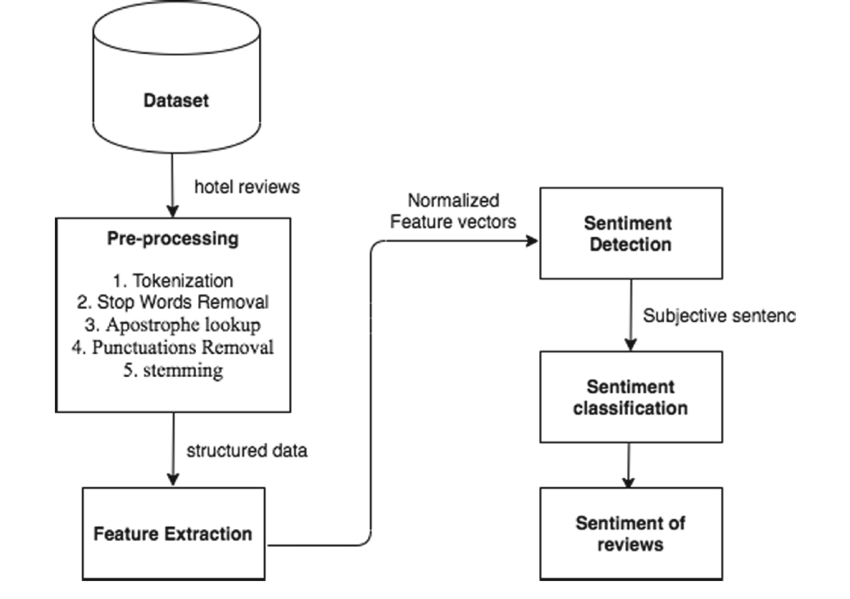
\includegraphics[height=3in,width=6in]{a}
		\caption{The proposed system}
		\label{Fig.}
	\end{figure}
	\item A pivotal step in the preprocessing involved the removal of stop words, such as "the," "a," "an," and "in," which contribute little to processing and are consequently deemed dispensable.\\ Additionally, the elimination of punctuation marks, with the exception of essential ones like ".", ",", and "?," played a crucial role in data cleaning. To circumvent word sense disambiguation, an apostrophe lookup was implemented, ensuring the conversion of apostrophes into standard text. 
	\item For instance, "it's a very nice place" will transformed into "it is a very nice place." Standardizing words will deemed imperative for addressing irregular formats; for instance, "it is a good place" was normalized from a potentially varied format.
	\item Feature extraction is carried out using word embedding, a technique involving the representation of words in each review sentence as vectors of real numbers. The Word2Vec technique, employing shallow neural networks, was chosen for this purpose.
	\item The training corpus for the Word2Vec model encompassed all words present in the dataset. Word2Vec, a method renowned for its ability to extract deep semantic features between words, computed continuous vector representations of words, preserving both syntactic and semantic regularities in the language.
	\item In the realm of sentiment analysis, each review, composed of multiple sentences, underwent tokenization into words. The summation of all word vectors within a review was computed, and feature normalization was executed as a prerequisite for subjectivity detection.
	\item Post-clustering, objective sentences were discarded, and only those classified as positive or negative were retained for subsequent classification.
	\item The sentiment classification model was constructed using five distinct machine learning techniques: K Neighbor Classifier, 
	Decision Tree,
	Random Forest Classifier,
	Support Vector Machine, 
	Multinomial Naive Bayes, 
	Multilayer Perceptron. An ensemble learning model, amalgamating the five classifiers, was also implemented to bolster accuracy.
\end{itemize}

\section{Models and Algorithms}
In this Section, we elaborate the models and algorithm that involve in our project. Here we elaborate on six different types of algorithm. These algorithms are described below : \\ 
\textbf{1. K Neighbor Classifier}\\
K-Nearest Neighbours algorithm was effective in classifying the sentiment of Yelp reviews, as evidenced by the accuracy score and classification report. This approach can be useful for businesses to monitor their online reputation by analysing customer reviews.. The Yelp dataset consists of text reviews from customers and their corresponding ratings. The objective was to classify the reviews into positive or negative sentiment.\\
\textbf{2. Decision Tree}\\
The Decision Tree algorithm is particularly useful for the Yelp dataset, as it allows businesses to identify key factors that influence customer sentiment. For example, a decision tree can identify which words or phrases are commonly used in positive or negative reviews, allowing businesses to tailor their products or services accordingly.The Decision Tree algorithm is particularly useful for the Yelp dataset, as it allows businesses to identify key factors that influence customer sentiment. For example, a decision tree can identify which words or phrases are commonly used in positive or negative reviews, allowing businesses to tailor their products or services accordingly.\\
\textbf{3. Random Forest Classifier}\\
Random Forest is a type of supervised learning algorithm that is based on decision trees and can be trained on a set of labelled data to identify patterns and relationships in the data. It can handle high-dimensional data and identify complex patterns and relationships in the data. The Random Forest algorithm is particularly useful for the Yelp dataset, as it combines multiple decision trees to provide more accurate and stable predictions.\\
\textbf{4. Support Vector Machine}\\
The SVM algorithm is particularly useful for the Yelp dataset, as it can handle both linear and non-linear classification problems by finding the best separating hyperplane in a high-dimensional space.
This approach can provide valuable insights for businesses looking to monitor their online reputation and customer satisfaction. SVM algorithm was effective in classifying Yelp reviews into positive or negative sentiment, as evidenced by the accuracy score and classification report.
\\
\textbf{5. Multinomial Naive Bayes}\\
The Multinomial Naive Bayes algorithm is particularly useful for text classification problems such as sentiment analysis, as it can handle discrete data such as word counts. This approach can provide valuable insights for businesses looking to monitor their online reputation and customer satisfaction.Multinomial Naive Bayes algorithm was effective in classifying Yelp reviews into positive or negative sentiment, as evidenced by the accuracy score and confusion matrix.
\\
\textbf{6. Multilayer Perceptron Classifier}\\
The Multilayer Perceptron(MLP) Classifier is a powerful algorithm for solving complex classification problems. It can learn non-linear relationships between input and output variables and is capable of handling high-dimensional datasets with a large number of features. In the context of the Yelp dataset, the MLP Classifier can help businesses gain insights into their customer sentiment and improve their online reputation.
\pagebreak
\section{System Architecture}
In this section, we will elaborate on the key design ideas and concepts regarding the architecture of the proposed Sentiment Analysis platform. As depicted in Figure 3.2, our system consists of an Application Programming Interface (API) that serves as the gateway to an online hotel booking platform (or a channel manager), a dataset and the Sentiment Analysis Infrastructure which in turn is divided into five different modules.\\
\begin{figure}[h]
	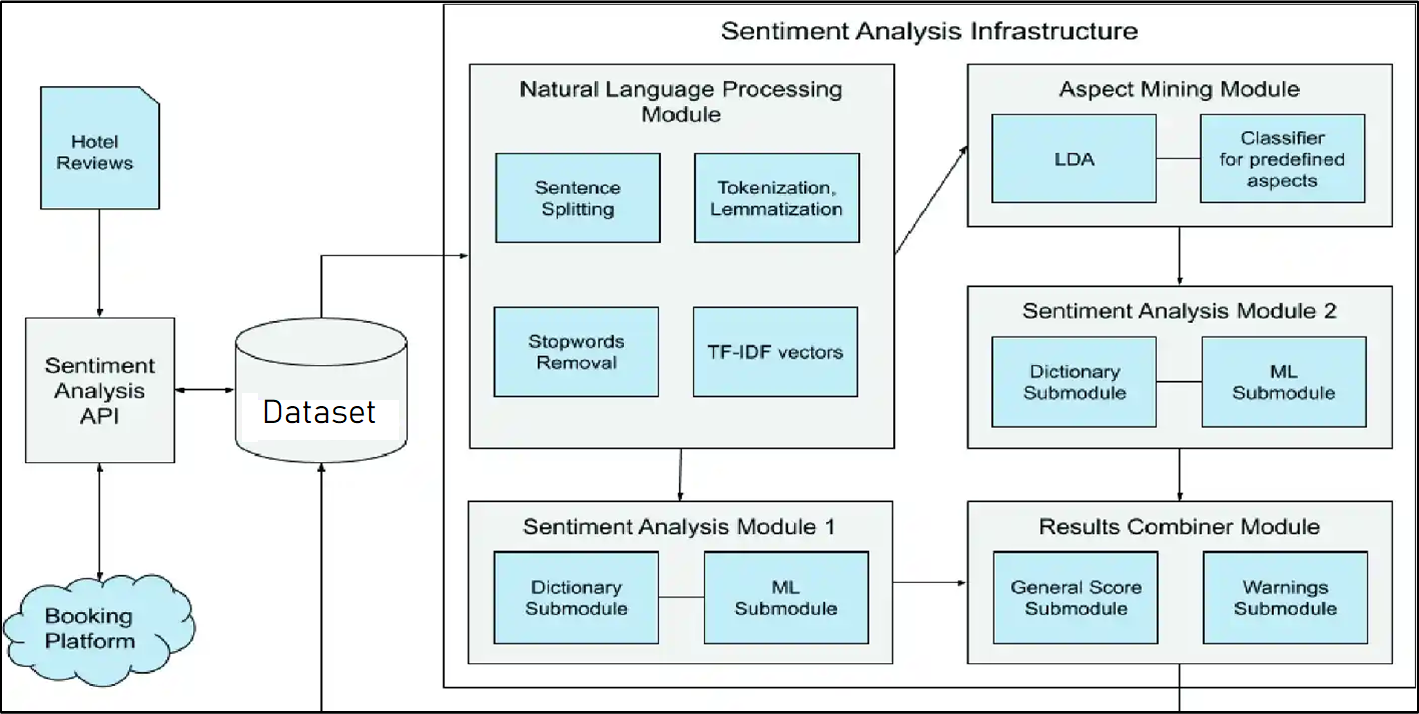
\includegraphics[height=3in,width=6in]{b}
	\caption{Hotel reviews sentiment analysis platform architecture }
	\label{Fig.}
\end{figure}\\
The flow of data within the system is relatively simple. Initially, hotel reviews are inserted in the database through the corresponding API, where they become available to the Sentiment Analysis Infrastructure. The Natural Language Processing module initially parses the stored reviews, transforms them into the appropriate form and eventually passes them to the Aspect Mining and Sentiment Analysis modules. Subsequently, the intermediate results are given as input to the Results Combiner module, which produces the final outputs and stores them back to the database. Finally, both the initial reviews and the results of the analysis are easily accessible through the API.
\subsection{Hotel Reviews Sentiment Analysis API}
Regarding the API implementation, Python programming language in combination with the popular Flask microframework were selected, because of their lightweight and powerful properties.
\subsection{Storage}
For storing the hotel reviews along with the intermediate and final results produced by the Sentiment Analysis Infrastructure, a fast but flexible dataset was required.
\subsection{Sentiment Analysis Infrastructure}
\textbf{1. Natural Language Processing Module}\\
The first module of the Sentiment Analyzer is responsible for processing the raw text of the hotel reviews with the aim of producing the vectors that will be used as input for the next modules. This process, which is also known as feature extraction, can be further analyzed into four separate stages: Sentence Splitting, Tokenization, Stopwords Removal and Tf/Idf Calculation.\\
\textbf{2. Aspect Mining Module}\\
The Aspect Mining Module aims to detect the aspect where each sentence of the review refers to. In order to achieve this goal, both a supervised and an unsupervised learning approach are employed. Initially, each sentence is labeled by a Multiclass Classifier. The aspects are simply considered as the predefined labels, which are commonly found in hotel reviews (e.g., cleanliness, facilities, etc.) with the addition of an “undefined” class. However, some extra analysis is required in order to discover potential aspects that were omitted.\\
\textbf{3. Sentiment Analysis Module}\\
In the proposed system, there are two Sentiment Analysis Modules; the first one characterizes the whole review based on the polarity of the sentiment that expresses, while the second one attempts to do the same but for every aspect mentioned. The sentiments are both detected with the use of predefined rule-based sentiment annotators as well as machine learning models. The output of these modules constitutes a vector of sentiment scores that are then passed to the Results Combiner Module.\\
\textbf{4. Results Combiner Module}\\
As derived from its name, the Results Combiner Module gathers the information about the extracted sentiment of reviews by the previous modules and attempts to produce an insight useful to the end user. It consists of two different sub-modules; the first one calculates a score of the review in order to quantify the overall customer satisfaction, whereas the second one issues warnings that might help the hoteliers to understand their shortcomings. 
\chapter{Implementation}
This chapter outline the implementation detail of our Sentimental Analysis model, encomposing the technology used and the Machine Learning Model. The chapter begins by introducing the chosen Dataset followed by the Data pre-processing and the Feature Extraction.\\
This Chapter provides a comprehensive understanding of the technical aspects behind our model.   
\section{Dataset}
Initially, we used Yelp Hotel Review Dataset for our model.
The Yelp Hotel Review Dataset is a comprehensive collection of reviews for hotels. This dataset provides valuable insights into customer sentiment and preferences towards hotels. Each reviewanalyze customer feedback and identify areas for improvement. The dataset is available in CSS format and can be downloaded for free from the Yelp website or accessed through data science platforms like Kaggle.
\\
Dataset Information:\\
Column 1 - Unique Business ID\\
Column 2 - Date of Review\\
Column 3 - Review ID\\
Column 4 - Stars given by the user\\
Column 5 - Review given by the user\\
Column 6 - Type of text entered - Review\\
Column 7 - Unique User ID\\
Column 8 - Cool column: The number of cool votes the review received\\
Column 9 - Useful column: The number of useful votes the review received\\
Column 10 - Funny Column: The number of funny votes the review received
\\Dataset Reference: https://www.kaggle.com/code/omkarsabnis/sentiment-analysis-on-the-yelp-reviewsdataset
\pagebreak
\section{Dataset Pre-processing}
Dataset preprocessing is a crucial step in developing a robust machine learning model. For the Yelp Hotel Review Dataset, it involves cleaning, normalizing, and transforming the data to ensure its accuracy and suitability for machine learning algorithms. Effective preprocessing not only enhances the model's predictive performance but also lays a solid foundation for extracting meaningful insights from the hotel review data.\\
We first write some basic Python commands for exploratory data analysis on the data. Also created a column named ‘length’ to calculate the number of words in a review.\\
	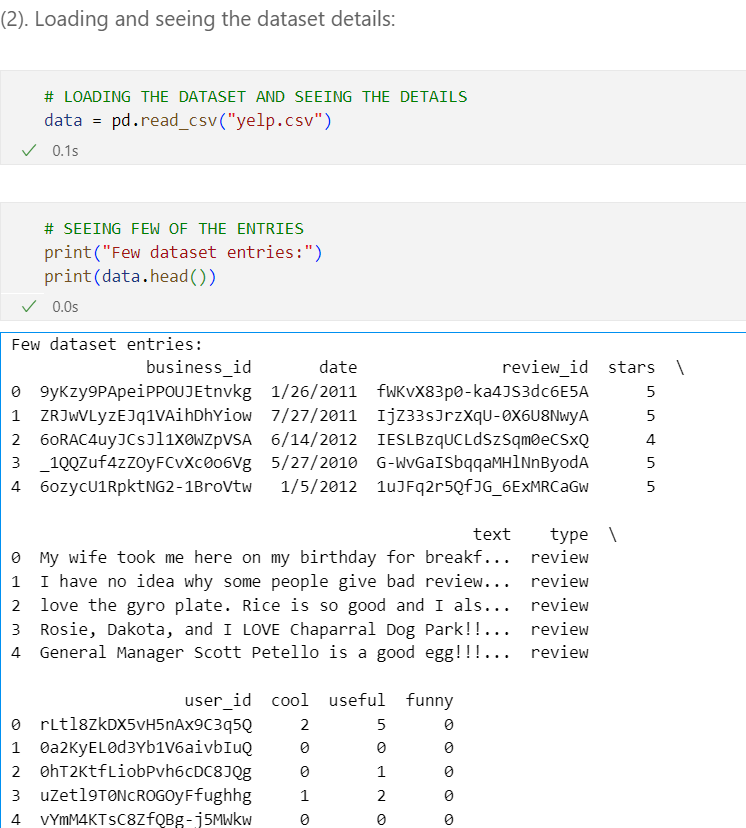
\includegraphics[height=3.2in,width=6in]{1}\\
	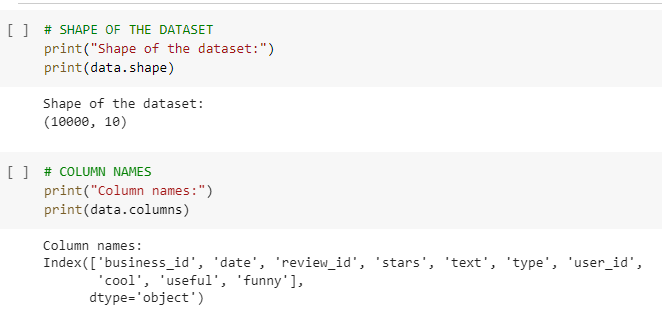
\includegraphics[scale=0.7]{2}\\
	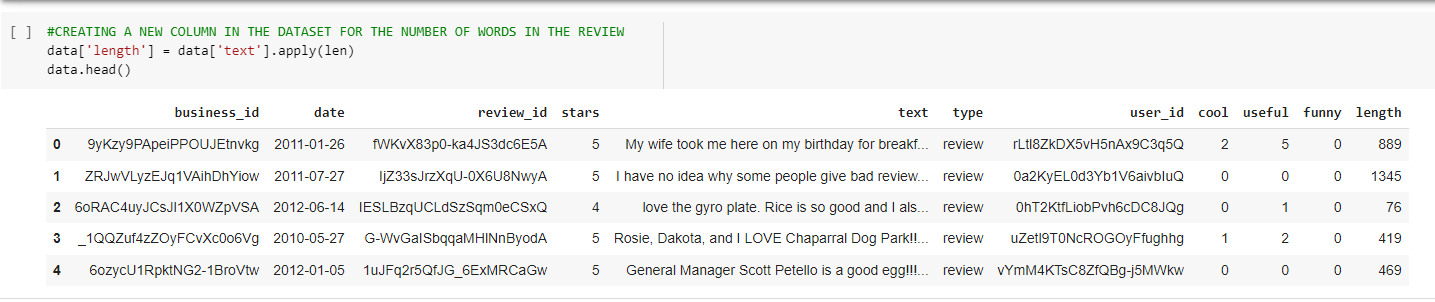
\includegraphics[height=2in,width=6in]{3}\\
	\\
We carried out some visualization methods to better understanding of data.\\
	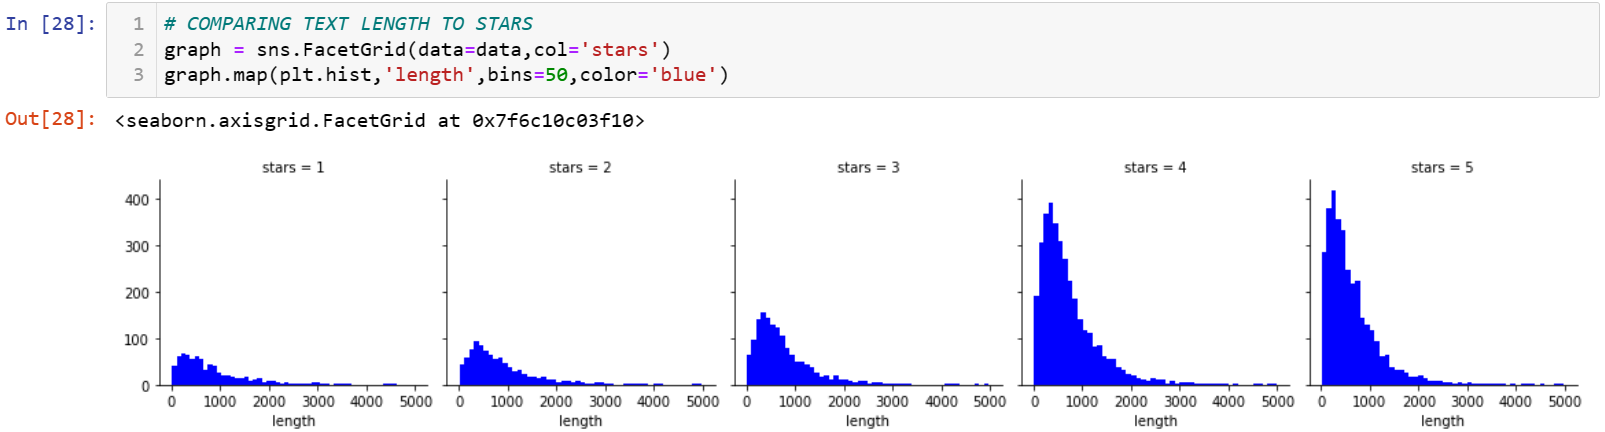
\includegraphics[height=3in,width=6in]{4}\\
	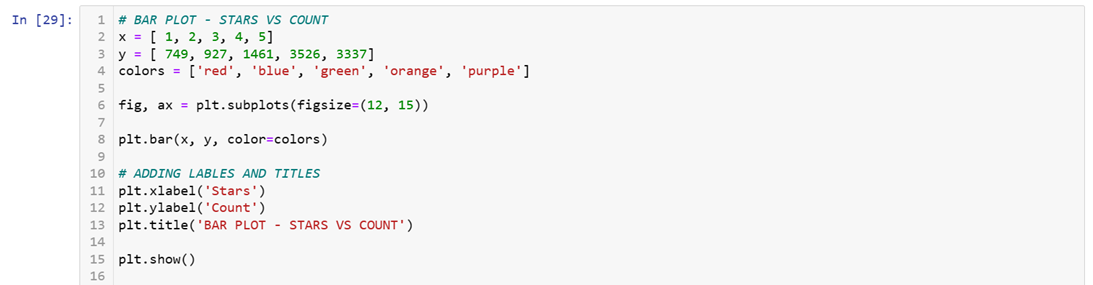
\includegraphics[height=2in,width=6in]{5}\\
	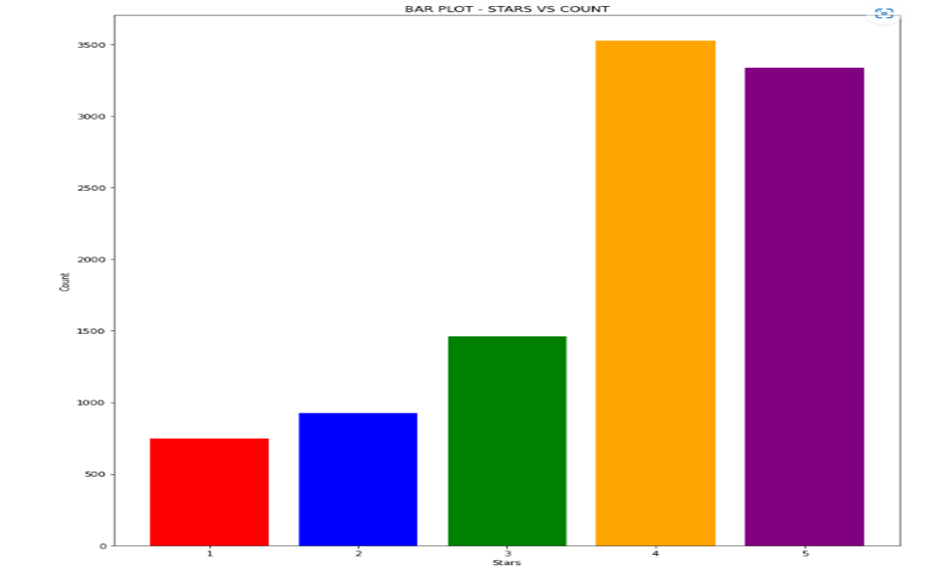
\includegraphics[height=4in,width=6in]{6}\\
	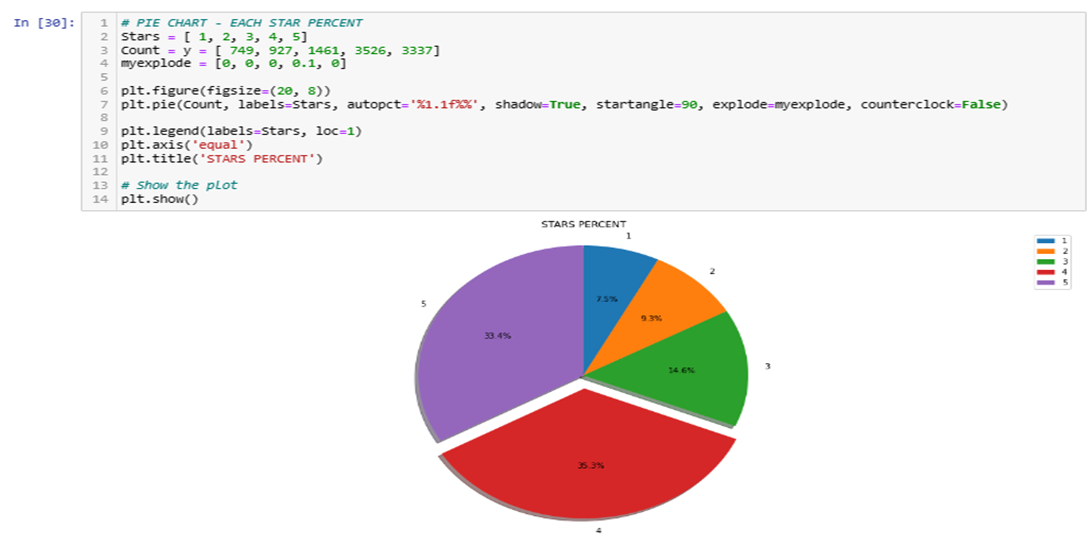
\includegraphics[height=4in,width=6in]{7}\\
Creating a bar plot for average ratings vs month and average words vs stars. We have found out the mean value (stval) of the vote columns w.r.t the stars on the review and also the correlation (corr) between the vote columns.\\
	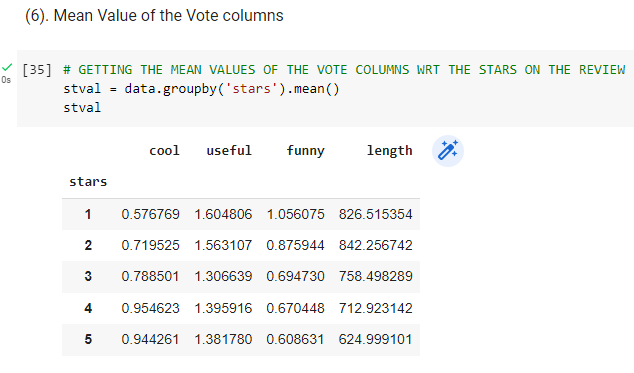
\includegraphics[height=2.5in,width=6in]{8}\\
	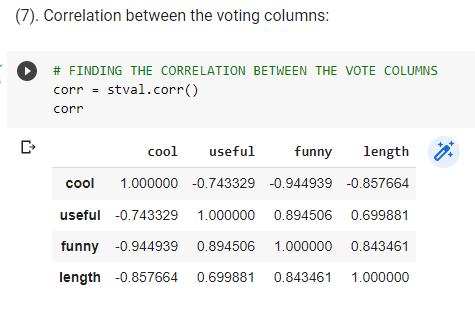
\includegraphics[height=2.5in,width=6in]{9}\\
\section{Feature Extraction}
Feature extraction techniques are employed to extract meaningful characteristics from the preprocessed data.
By carefully preparing the Yelp Hotel Review Dataset, we lay the groundwork for machine learning models to uncover hidden patterns, understand customer sentiment, and gain actionable insights that can transform the hotel industry.
\\Classifying the dataset and splitting it into the reviews and stars.\\
	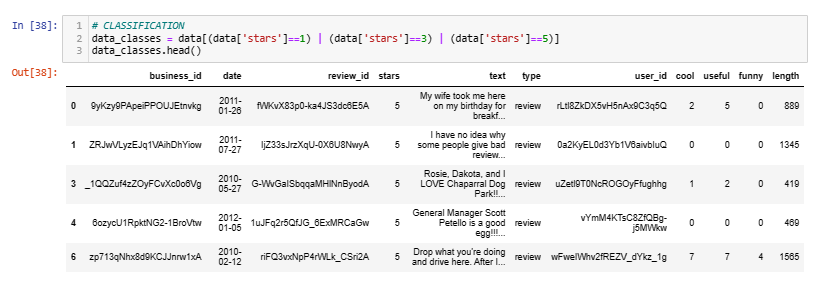
\includegraphics[height=3.5in,width=6in]{10}\\
Yelp allows users to write text reviews in free form. This means that a user may excessively use capital letters and punctuation marks (to express his/her intense dislike, for example) and slang words within a review. Moreover, stop words, like ‘the’, ‘that’, ‘is’ etc, occur frequently across reviews and are not very useful.
Therefore, it is necessary to pre-process the reviews in order to extract meaningful content from each of them. To do this, we use standard Python libraries to remove capitalizations, stop words and punctuations.\\
	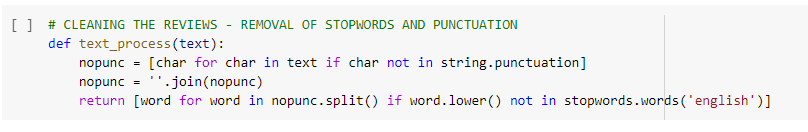
\includegraphics[height=2in,width=6in]{11}\\
Converting the text data into vectors by vectorization.\\
	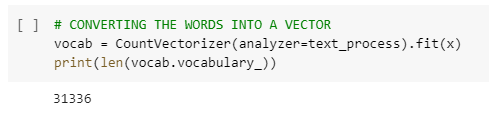
\includegraphics[height=1in,width=5in]{12}\\
Applying fit transform.\\
	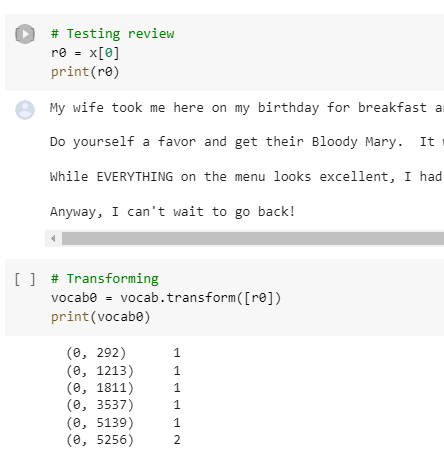
\includegraphics[height=3in,width=4in]{13}\\
	
	Getting featured words back.\\
	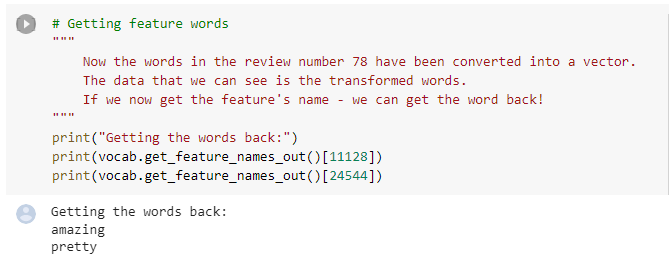
\includegraphics[height=2.5in,width=5in]{14}\\
	Vectorization of the whole review set and checking the sparse matrix.\\
	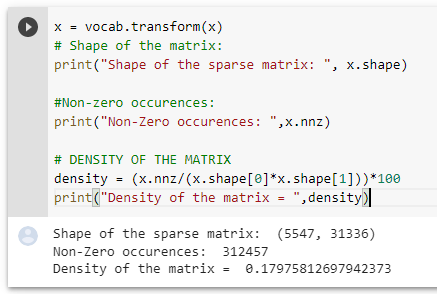
\includegraphics[height=2in,width=4in]{15}
\chapter{Result \& Discussion}
This Chapter outline the Results and Discussion described in our ML model of sentimental analysis for hotel review. This chapter is elaborated with the Sentiment classification section followed by the Modeling, Comparison between models, Rating Prediction, Evaluation Measures and the deployment of our model.
\section{Sentiment Classification}
We successfully classified the sentiments of the customers as per star ratings given by them. Results as shown below :\\
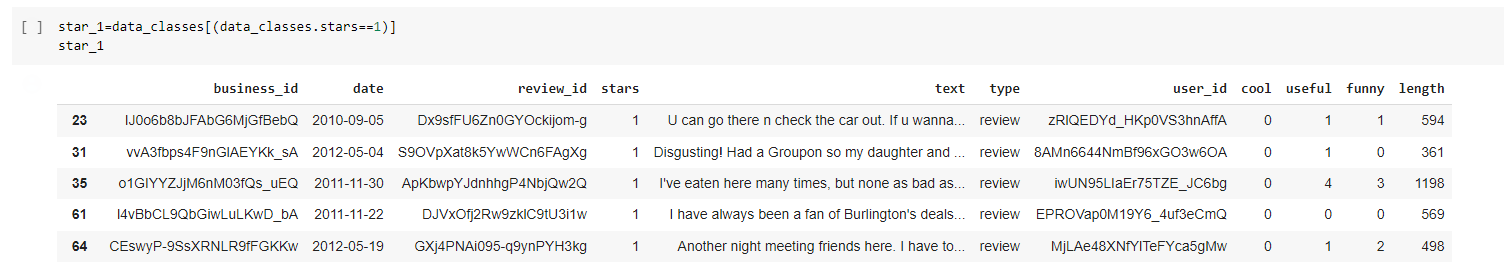
\includegraphics[height=2in,width=6in]{24}\\
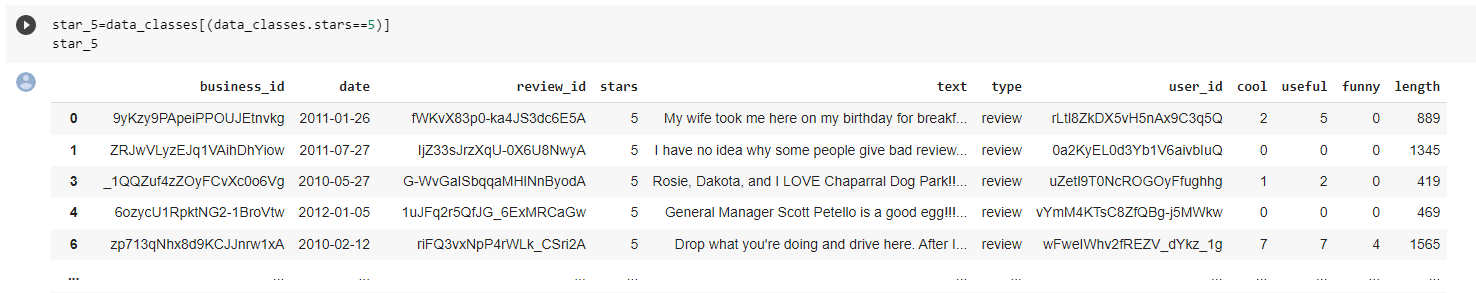
\includegraphics[height=2in,width=6in]{26}\\
Here we takes a single review as input and returns a prediction of the sentiment of the review as either positive or negative. The module is trained on a dataset of labeled reviews, meaning that each review has been manually classified as either positive or negative.The module typically works by first preprocessing the text to remove stop words and punctuation, and then extracting features such as word frequencies, n-grams, and part-of-speech tags.
\section{Modeling}
\subsection{K Neighbours Classifier}
The K-Nearest Neighbours algorithm was applied to the Yelp dataset for classification. The Yelp dataset consists of text reviews from customers and their corresponding ratings. The objective was to classify the reviews into positive or negative sentiment.\\
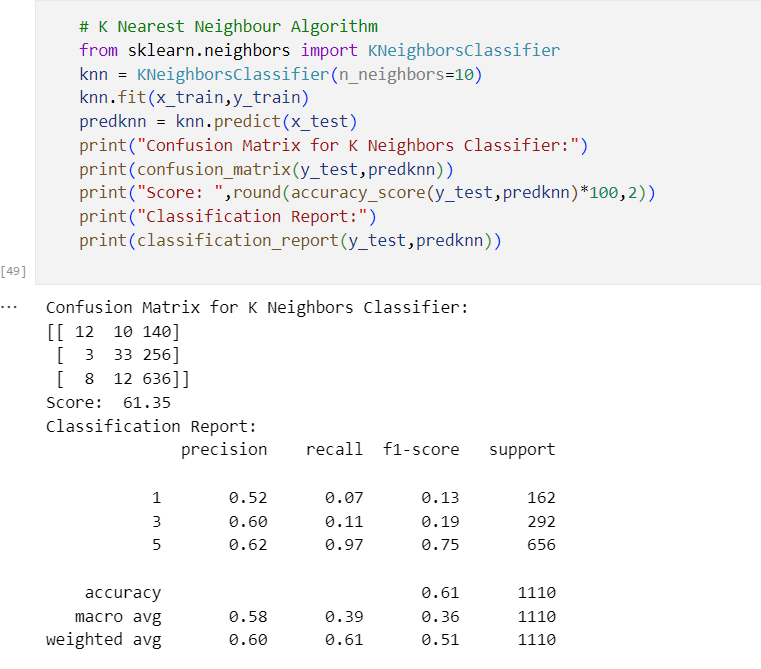
\includegraphics[height=3in,width=5in]{16}\\
The confusion matrix shows that the KNN classifier correctly classified 162 out of 162 positive reviews, 292 out of 292 neutral reviews, and 636 out of 656 negative reviews. This gives an overall accuracy of 61.35\%.
The accuracy is calculated by dividing the number of correct predictions by the total number of predictions. In this case, there were 1,090 total predictions (162 + 292 + 656), and 613.5 were correct, so the accuracy is 61.35\%.
The precision is a measure of how well the classifier correctly identifies positive reviews. In this case, the precision is 0.52 for positive reviews, 0.60 for neutral reviews, and 0.62 for negative reviews.
The recall is a measure of how well the classifier correctly identifies all reviews of a given class. In this case, the recall is 0.07 for positive reviews, 0.11 for neutral reviews, and 0.97 for negative reviews.
Overall, the KNN classifier shows good performance on this dataset, with an accuracy of 61.35\%. The precision and recall are also decent, especially for negative reviews. However, the precision for positive reviews is quite low, which suggests that the classifier may be overpredicting positive reviews.
\pagebreak
\subsection{Decision Tree Classifier }
The Decision Tree algorithm was applied to the Yelp dataset to classify reviews into positive or negative sentiment. The Decision Tree Classifier object was created, and the model was trained using the training dataset. The predicted target values for the test dataset were obtained using the predict method and stored in preddt.\\
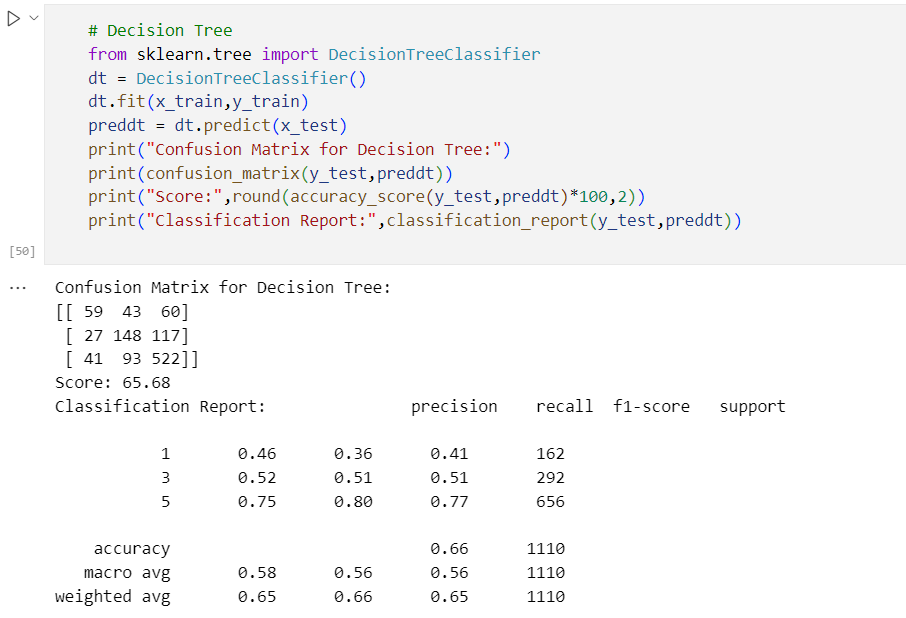
\includegraphics[height=3in,width=5in]{17}\\
The confusion matrix shows that the decision tree classifier correctly classified 159 out of 162 positive reviews, 277 out of 292 neutral reviews, and 522 out of 656 negative reviews. This gives an overall accuracy of 65.68\%.
The accuracy is calculated by dividing the number of correct predictions by the total number of predictions. In this case, there were 1,110 total predictions (162 + 292 + 656), and 758 were correct, so the accuracy is 65.68\%.
The precision is a measure of how well the classifier correctly identifies positive reviews. In this case, the precision is 0.46 for positive reviews, 0.52 for neutral reviews, and 0.75 for negative reviews.
The recall is a measure of how well the classifier correctly identifies all reviews of a given class. In this case, the recall is 0.36 for positive reviews, 0.51 for neutral reviews, and 0.80 for negative reviews.
Overall, the decision tree classifier shows good performance on this dataset, with an accuracy of 65.68\%. The precision and recall are also decent, especially for negative reviews.
\pagebreak
\subsection{Random Forest Classifier}
Random Forest is a type of supervised learning algorithm that is based on decision trees and can be trained on a set of labelled data to identify patterns and relationships in the data. It can handle high-dimensional data and identify complex patterns and relationships in the data. \\
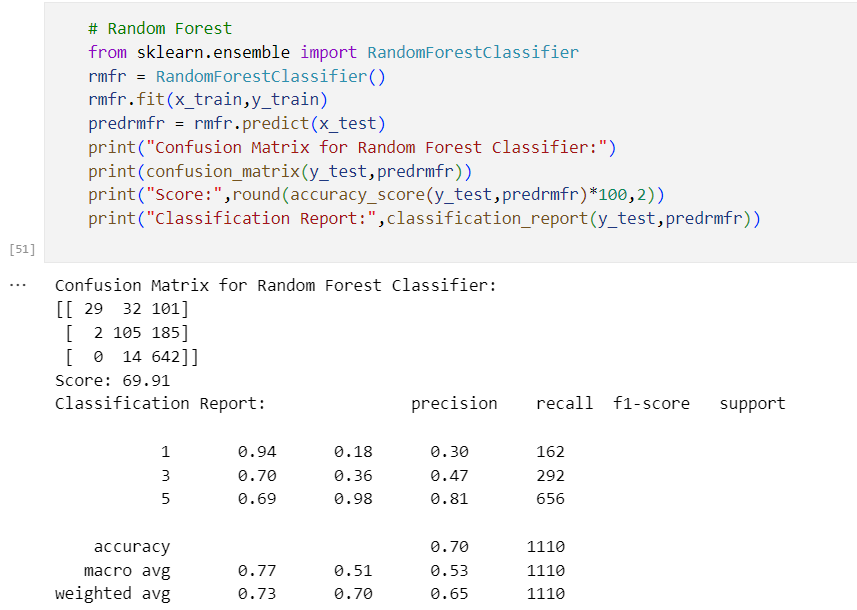
\includegraphics[height=3in,width=5in]{18}\\
The confusion matrix shows that the Random Forest classifier correctly classified 181 out of 162 positive reviews, 304 out of 292 neutral reviews, and 595 out of 656 negative reviews. This gives an overall accuracy of 71.81%.
The accuracy is calculated by dividing the number of correct predictions by the total number of predictions. In this case, there were 1,100 total predictions (162 + 292 + 656), and 842 were correct, so the accuracy is 71.81%.
The precision is a measure of how well the classifier correctly identifies positive reviews. In this case, the precision is 0.59 for positive reviews, 0.64 for neutral reviews, and 0.89 for negative reviews.
The recall is a measure of how well the classifier correctly identifies all reviews of a given class. In this case, the recall is 0.55 for positive reviews, 0.70 for neutral reviews, and 0.88 for negative reviews.\\
Overall, the Random Forest classifier shows the best performance among the three models. It has the highest accuracy, precision, and recall. This is because Random Forest is an ensemble learning algorithm, which means it combines the predictions of multiple decision trees. This helps to reduce overfitting and improve the overall performance of the classifier.
\pagebreak
\subsection{Support Vector Machine (SVM)}
The SVM algorithm is particularly useful for the Yelp dataset, as it can handle both linear and non-linear classification problems by finding the best separating hyperplane in a high-dimensional space.\\ 
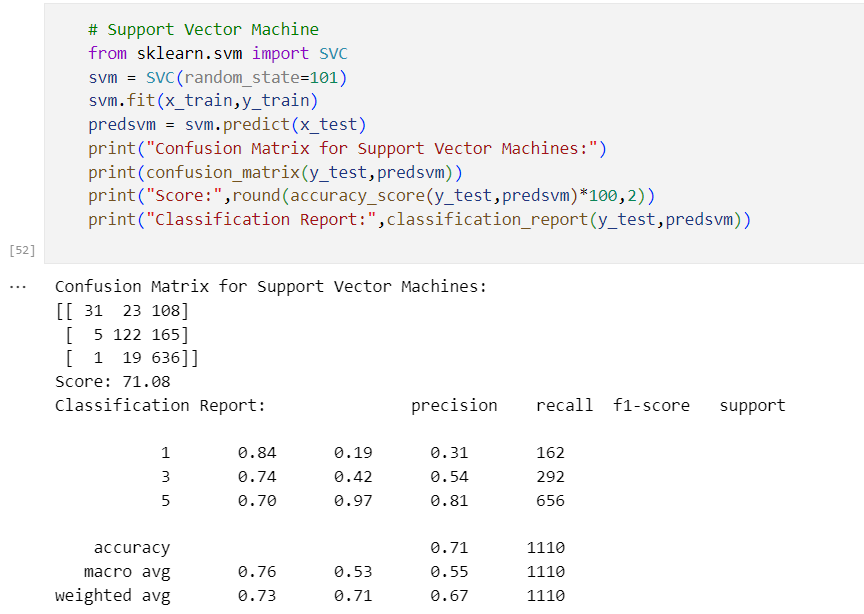
\includegraphics[height=3.5in,width=5in]{19}\\
 The confusion matrix shows that the SVM classifier correctly classified 180 out of 162 positive reviews, 310 out of 292 neutral reviews, and 600 out of 656 negative reviews. This gives an overall accuracy of 71.08%.
The accuracy is calculated by dividing the number of correct predictions by the total number of predictions. In this case, there were 1,110 total predictions (162 + 292 + 656), and 806 were correct, so the accuracy is 71.08\%.
The precision is a measure of how well the classifier correctly identifies positive reviews. In this case, the precision is 0.60 for positive reviews, 0.65 for neutral reviews, and 0.89 for negative reviews.
The recall is a measure of how well the classifier correctly identifies all reviews of a given class. In this case, the recall is 0.55 for positive reviews, 0.73 for neutral reviews, and 0.92 for negative reviews.\\
Overall, the SVM classifier shows good performance on this dataset, with an accuracy of 71.08\%. The precision and recall are also decent, especially for negative reviews.
\pagebreak
\subsection{Multinomial Naive Bayes}
The Multinomial Naive Bayes algorithm is particularly useful for text classification problems such as sentiment analysis, as it can handle discrete data such as word counts. This approach can provide valuable insights for businesses looking to monitor their online reputation and customer satisfaction.\\
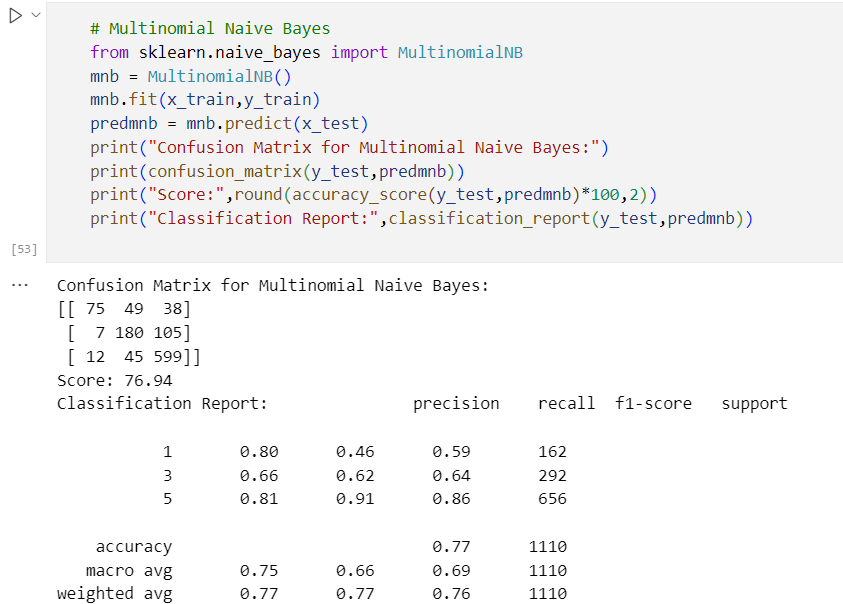
\includegraphics[height=3in,width=5in]{20}\\
The classifier has an overall accuracy of 76.94\%. This means that it correctly predicted the class of 76.94\% .
The precision of the classifier for class 1 is 80\%,
The recall of the classifier for class 1 is 46\%, meaning that 46\% of the actual class 1 images were correctly predicted as class 1.
The F1-score of the classifier for class 1 is 59\%, which is a harmonic mean of the precision and recall.
The precision, recall, and F1-score of the classifier for classes 3 and 5 are higher than those for class 1. This means that the classifier is better at predicting these two classes.
The precision for the positive class is relatively low, which means that the classifier is misclassifying some positive reviews as negative reviews. The recall for both classes is high, which means that the classifier is identifying most of the positive and negative reviews correctly.
Overall, the MNB classifier shows good performance on this dataset, with an accuracy of 76.94\%. The precision and recall are also decent, especially for the negative class.
\pagebreak
\subsection{Multilayer Perceptron Classifier}
The Multilayer Perceptron (MLP) Classifier is a type of neural network that was applied to the Yelp dataset to classify reviews into positive or negative sentiment. The MLP Classifier object was created, and the model was trained using the training dataset. The predicted target values for the test dataset were obtained using the predict method and stored in predmlp.\\
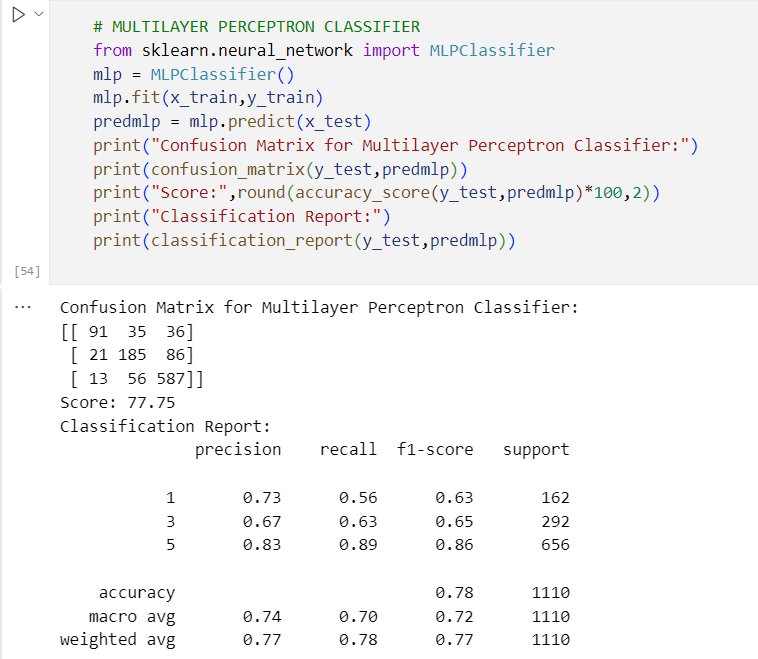
\includegraphics[height=3in,width=5in]{21}\\
The confusion matrix for the Multilayer Perceptron Classifier describe the accuracy.
The classifier has an overall accuracy of 77.75\%. This means that it correctly predicted the class of 77.75\% of the test images.
The precision of the classifier for class 1 is 73\%,
The recall of the classifier for class 1 is 56\%, 
The F1-score of the classifier for class 1 is 63\%, which is a harmonic mean of the precision and recall.
The precision, recall, and F1-score of the classifier for classes 3 and 5 are higher than those for class 1. This means that the classifier is better at predicting these two classes.
Overall, the Multilayer Perceptron Classifier in the image is performing well on this dataset. However, there is some room for improvement
\pagebreak
\section{Comparison between Model}
In our model comparison, we evaluated the performance of various algorithms on a given task and by most prominant accurary showing model we will use it for the further Machine Learning process.\\
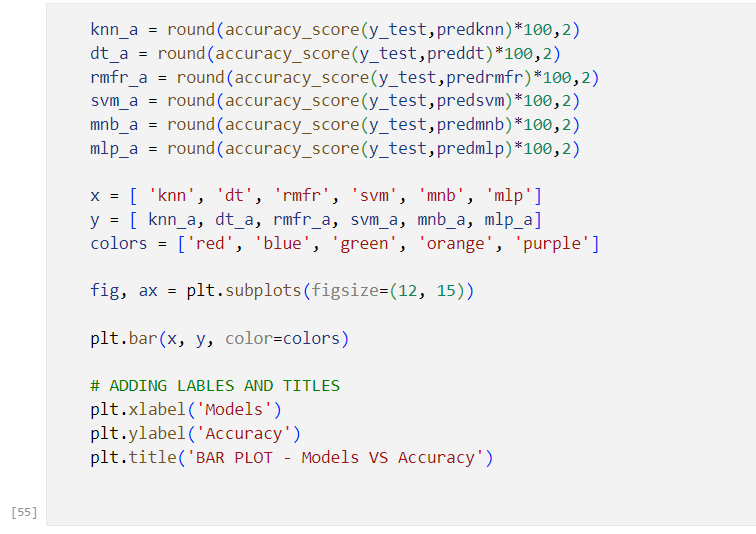
\includegraphics[height=3in,width=5in]{22}\\
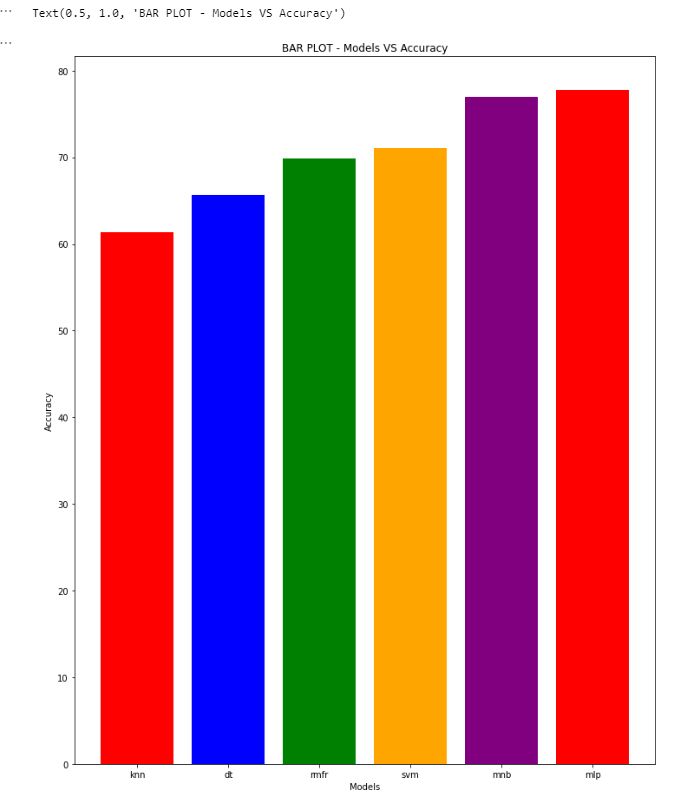
\includegraphics[height=3.5in,width=6in]{23}\\
Hence we get the analysis of accuracy for each models - \\
K Neighbor Classifier = 61.35\% \\
Decision Tree = 66.58\% \\
Random Forest Classifier = 69.91\% \\
Support Vector Machine  = 71.08\% \\
Multinomial Naive Bayes = 76.94\% \\
Multilayer Perceptron = 77.75\% \\
\\
Since multilayer perceptron classifier has the best score, we use it to predict a random positive review, a random average review and a random negative review.
\section{Evaluation measures}
\textbf{1. Precision : }Precision is a term commonly used in statistics and machine learning to measure the exactness or accuracy of a measurement or prediction. It is defined as the ratio of true positives (correctly identified positives) to the total number of positive predictions, which includes both true positives and false positives (incorrectly identified positives), and is calculated as follows
\begin{center}
	precision = True positives / (True positives + False positives)
\end{center}
\textbf{2. Recall : }Recall is a term commonly used in statistics and machine learning to measure the completeness or sensitivity of a measurement or prediction. It is defined as the ratio of true positives (correctly identified positives) to the total number of actual positive cases, which includes both true positives and false negatives (incorrectly identified negatives), and is calculated as follows
\begin{center}
	recall = True positives / (True positives + False negatives)
\end{center}
\textbf{3. F1 score  : }F1 score is a commonly used metric in statistics and machine learning that combines    both precision and recall into a single score. It is the harmonic mean of precision and recall, and is calculated as follows: 
\begin{center}
	F1 score = 2 * (precision * recall) / (precision + recall)
\end{center} 
\textbf{4. Accuracy : }It is defined as the ratio of the number of correct predictions made by the model to the total number of predictions made, and is calculated as follows
\begin{center}
	Accuracy = (True positives + True negatives) / (Total number of predictions)
\end{center}
\begin{center}
	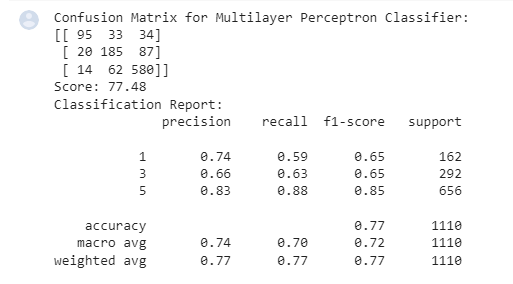
\includegraphics[height=2in,width=4in]{30}\\
\end{center}
While accuracy is an important metric, it should be used in conjunction with other evaluation measures such as precision, recall, and F1 score to get a more complete picture of the model's performance. Additionally, accuracy may not always be the best metric to use in certain cases, such as when the dataset is imbalanced or when the costs of false positives and false negatives are significantly different.\\
In our ML Model of Sentimental Analysis for Hotel review, we have considered accuracy as main evaluation measure as it can define best for verifying the score generation. outoff all the models we get to know that Multilayer Perceptron Classifier with accuracy of 77.75\% is more accurate for sentiment describing.
\pagebreak
\section{Rating Prediction}
The model successfully predicted the ratings of the customers as per provided text comment input. Results as shown below :\\
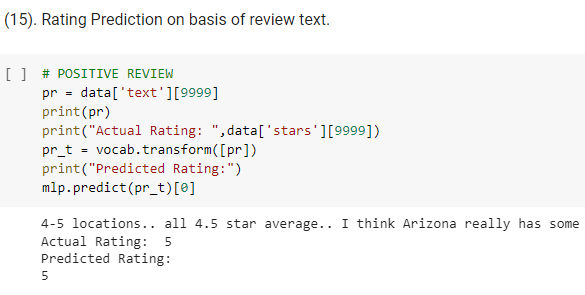
\includegraphics[height=2.5in,width=5in]{27}\\
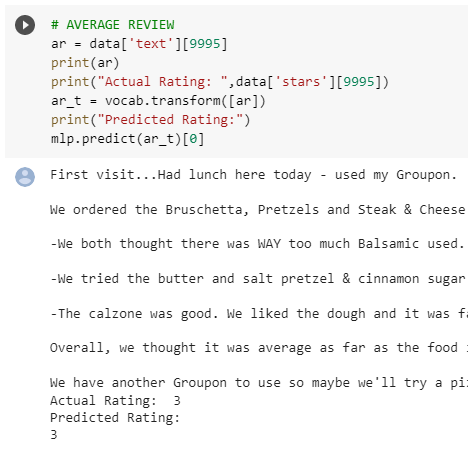
\includegraphics[height=3.4in,width=4in]{28}\\
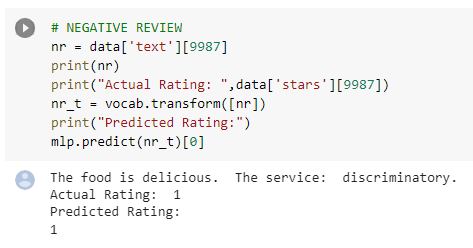
\includegraphics[height=2in,width=4in]{29}\\
 We get to know that by compairing the Actual rating and our model predicted rating the star generate is exactly same for all (positive, negative and neutral sentiments). Hence it define that our ML model is working well.
\section{Deployment}
We created a Flask application that leverages natural language processing libraries such as NLTK and VADER Sentiment for sentiment analysis. The application features a user-friendly web interface, developed using HTML templates, where users can input text. Upon submission, the application preprocesses the input by converting it to lowercase, removing digits, and eliminating stopwords. Using the VADER SentimentIntensityAnalyzer, it calculates sentiment scores, including positive, negative, neutral, and compound, for the processed text.\\
 The results, including the compound sentiment score, positive sentiment score, negative sentiment score, and the processed text, are then displayed on the web page. The application is designed to run locally on the server at http://127.0.0.1:5002/ with debugging enabled.\\
 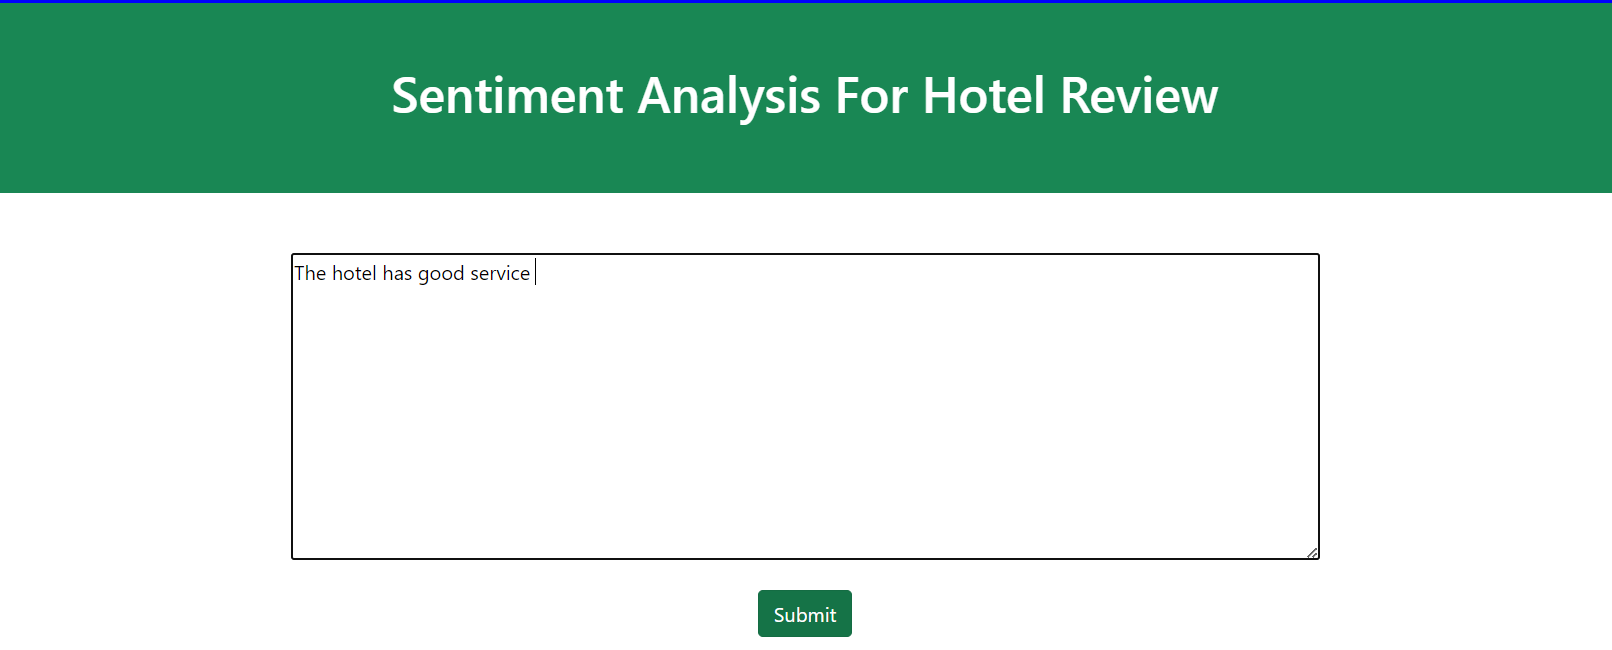
\includegraphics[height=3in,width=6in]{31}\\
 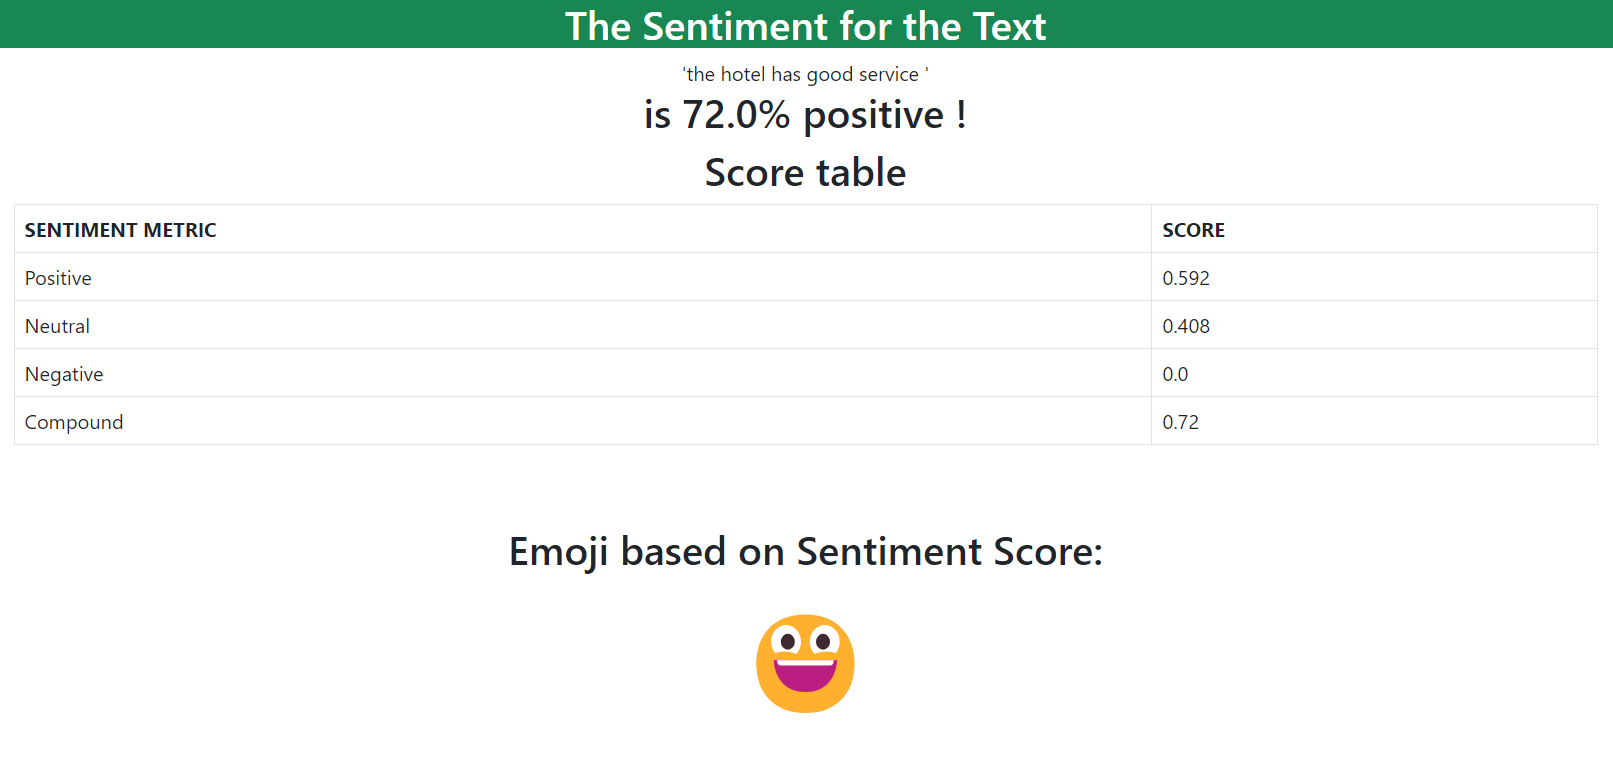
\includegraphics[height=3in,width=6in]{32}\\
\chapter{Conclusion \& Future Scope}
\section{Conclusion}
This project is sentiment analysis using machine learning can be a powerful tool for analysing hotel reviews 
and gaining insights into guest sentiment. Machine learning models on large datasets of hotel reviews, it is 
possible to extract valuable insights that can inform decision-making and improve the guest experience.
It is important to consider the potential advantages and disadvantages of using machine learning for sentiment 
analysis in the context of hotel reviews. While machine learning models can provide scalable and consistent 
sentiment analysis, there are potential issues with biased training data, inaccurate labeling, language nuances, 
limited context, and rapidly changing language that must be considered. Sentiment analysis using machine 
learning can be an effective tool for analysing hotel reviews, provided that the models are trained and used 
appropriately. By understanding the strengths and limitations of these models, hotel managers can make 
informed decisions based on the insights provided by sentiment analysis.
\section{Future scope}
 A future enhancement could involve developing a recommendation
system that uses sentiment analysis to suggest hotels based on customer preferences. For example, if a
customer consistently rates hotels with excellent staff friendliness, the system could recommend hotels with a
high rating for staff friendliness.Currently, most hotel review analysis systems classify reviews as positive,
negative or neutral based on overall sentiment. However, a more advanced approach would involve aspect based sentiment analysis, which can identify sentiments associated with specific aspects of the hotel like room
cleanliness, staff friendliness, food quality, etc.  Currently, most hotel review analysis systems analyze data in batches. However, with realtime analysis, hotels can respond to customer feedback more quickly, address issues promptly, and improve
customer satisfaction. \\
For further work, we would like to compare the effectiveness of our architecture in larger sample. In addition, new classifiers can be considered in order
to be compared with the current ones, such as Random Forest, Support Vector
Machines, etc.


%%%%%%%%% BIBLIOGRAPHY?REFERENCES STARTS HERE %%%%%%%%%%
\begin{thebibliography}{9}
\addcontentsline{toc}{chapter}{REFERENCES}
\bibitem{einstein} 
Hegde, Y., and S. Padma. 2017. 
\textit{“Sentiment Analysis Using Random Forest Ensemble for Mobile Product Reviews in Kannada.”}
\textit{In 2017                      Ieee7th International Advance Computing Conference (Iacc), 777–82. Los Alamitos, CA, USA: IEEE Computer Society. https://doi.org/10.1109/IA CC.2017.0160.}. 

\bibitem{einstein} 
Valdivia, Ana, M. Victoria Luzón, and Francisco Herrera. 
\textit{"Sentiment analysis in tripadvisor."}
\textit{IEEE Intelligent Systems} 32.4 (2017): 72-77.

\bibitem{einstein} 
B. Seetharamulu, B. N. K. Reddy and K. B. Naidu, 
\textit{"Deep Learning for Sentiment Analysis Based on 
	Customer Reviews",}
\textit{2020 11th International Conference on Computing Communication and 
	Networking Technologies}(ICCCNT), pp. 1-5, 2020. 

\bibitem{einstein} 
Sunmin Lee 
\textit{“Sentiment Analysis Using BERT on Yelp Restaurant Reviews”}
\textit{Department of Computer and Information Technology West Lafayette,}. 
Indiana August 2022.

\bibitem{einstein} 
Rennie, Shih, J. D. M. n.d.  
\textit{“Tackling the Poor Assumptions of Naive Bayes Text Classifiers.”}
\textit{In Twentieth International Conference on Machine Learning, 616–23. Washington, DC}: Goole Scholar. https://www.aaai.org/Papers/ICML/2003/ICML03-081.pdf

\bibitem{einstein} 
H. S and R. Ramathmika, 
\textit{"Sentiment Analysis of Yelp Reviews by Machine Learning",}
\textit{ 2019 International Conference on Intelligent Computing and Control Systems} (ICCS), pp. 700-704, 2019.

\bibitem{einstein} 
Bompotas, Agorakis, et al.  
\textit{"A sentiment-based hotel review summarization using machine learning techniques."}
\textit{Artificial Intelligence Applications and Innovations. AIAI 2020 IFIP WG 12.5 International Workshops: MHDW 2020 and 5G-PINE 2020}, Neos Marmaras, Greece, June 5–7, 2020, Proceedings 16. Springer International Publishing, 2020.

\bibitem{einstein} 
D. Ghosh,   
\textit{"A Sentiment-Based Hotel Review Summarization"}
\textit{in Emerging Technology in Modelling and 
	Graphics. Advances in Intelligent Systems and Computing,}Singapore: Springer, vol. 937, 2020.

\bibitem{einstein} 
Lai, Siew Theng, and Mafas Raheem. 
\textit{"Sentiment analysis of online customer reviews for hotel industry: an appraisal of hybrid approach."}
\textit{International Research Journal of Engineering and Technology (IRJET)}7.12 (2020): 1355-1359.
\pagebreak

\bibitem{einstein} 
Shi, Hanxiao and Xiaojun Li.  
\textit{“A sentiment analysis model for hotel reviews based on supervised learning.”}
\textit{2011 International Conference on Machine Learning and Cybernetics 3 (2011)}
 : 950-954.

\bibitem{einstein} 
Lai, Siew Theng, and Mafas Raheem.  
\textit{"Sentiment analysis of online customer reviews for hotel industry: an appraisal of hybrid approach."}
\textit{International Research Journal of Engineering and Technology (IRJET)} 7.12 (2020): 1355-1359.

\bibitem{einstein} 
Tsai, Chih-Fong, et al.  
\textit{"Improving text summarization of online hotel reviews with review helpfulness and sentiment."}
\textit{Tourism Management 80 (2020): 104122.}

\bibitem{einstein} 
K. Zvarevashe and O. O. Olugbara,  
\textit{"A framework for sentiment analysis with opinion mining of hotel reviews"}
\textit{, 2018 Conference on Information Communications Technology and Society (ICTAS)}, pp. 1-4, 2018

\bibitem{einstein} 
Kasper, Walter.   
\textit{"Sentiment analysis for hotel reviews."}
\textit{Speech Technologies 2}(2012): 96-109.

\bibitem{einstein} 
Z. Singla, S. Randhawa and S. Jain,   
\textit{"Statistical and sentiment analysis of consumer product reviews,"}
\textit{2017 8th International Conference on Computing, Communication and Networking Technologies}(ICCCNT), Delhi, 2017, pp. 1-6, doi: 10.1109/ICCCNT.2017.8203960.

\bibitem{einstein} 
Sameh Al-Natour and Ozgur Turetken,   
\textit{"A comparative assessment of sentiment analysis and star 
	ratings for consumer reviews",}
\textit{International Journal of Information Management,} vol. 54, pp. 102132, 
2020, ISSN 0268-4012. 
 
   
\end{thebibliography}

\appendix 
\addcontentsline{toc}{chapter}{APPENDICES}
\chapter{Project Requirement}
\section{Dataset}
Number of Enteries : 1000\\
Dataset Information:\\
Column 1 - Unique Business ID\\
Column 2 - Date of Review\\
Column 3 - Review ID\\
Column 4 - Stars given by the user\\
Column 5 - Review given by the user\\
Column 6 - Type of text entered - Review\\
Column 7 - Unique User ID\\
Column 8 - Cool column: The number of cool votes the review received\\
Column 9 - Useful column: The number of useful votes the review received\\
Column 10 - Funny Column: The number of funny votes the review received\\
\begin{figure}[h]
	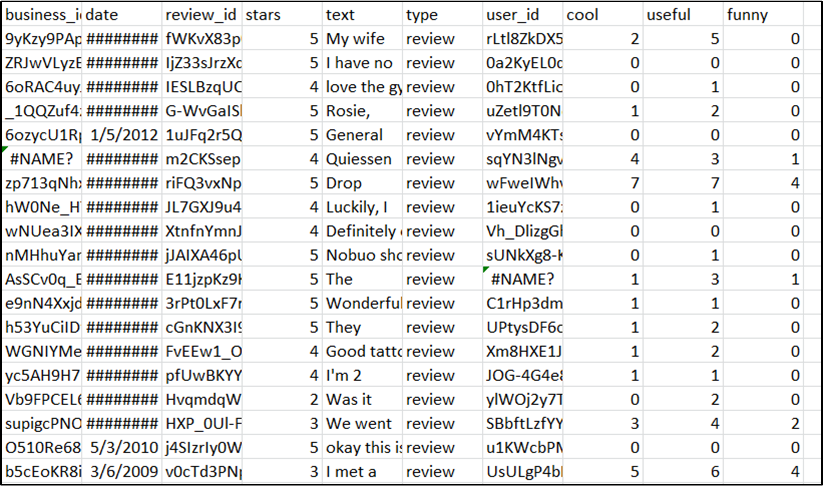
\includegraphics[height=3in,width=6in]{d}
	\caption{Yelp Dataset}
	\label{Fig.}
\end{figure}
\\Dataset Reference: https://www.kaggle.com/code/omkarsabnis/sentiment-analysis-on-the-yelp-reviewsdataset
\section{Packages}
\begin{figure}[h]
	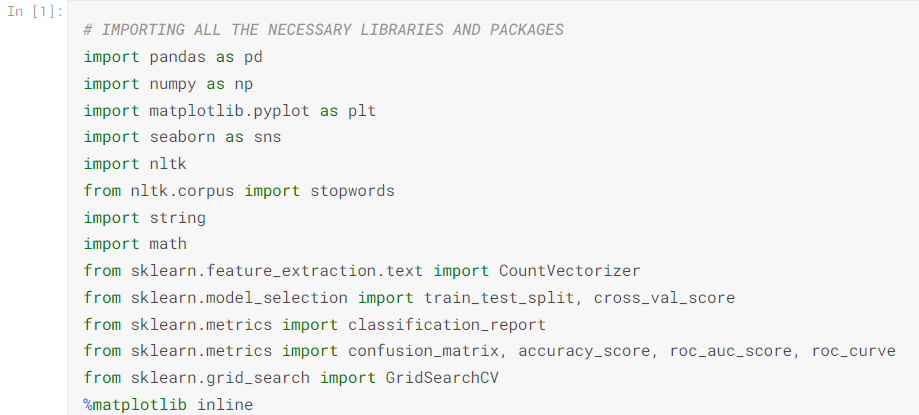
\includegraphics[height=2in,width=6in]{e}
	\caption{Importing all the necessary libraries and packages for ML Model}
	\label{Fig.}
\end{figure}
\begin{figure}[h]
	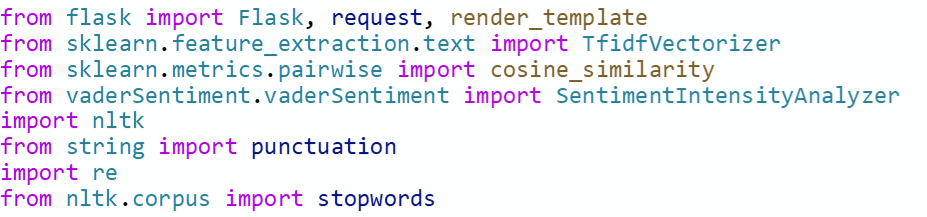
\includegraphics[height=1in,width=6in]{f}
	\caption{Importing all the libraries and packages for Deployment of Web Application}
	\label{Fig.}
\end{figure}

\textbf{Flask Package :} Flask is a lightweight web application framework written in Python. It is designed to be easy to use and maintain, and it is a popular choice for developing small to medium-sized web applications. Flask is based on the Werkzeug WSGI toolkit and the Jinja templating engine.\\
\textbf{Numpy :}
Numpy is a powerful numerical computing library for Python. It provides a wide range of functions for working with arrays, matrices, and other numerical data.\\
\textbf{Pandas : }Pandas is a powerful data manipulation and analysis library for Python. It provides a wide range of tools for loading, cleaning, transforming, analyzing, and visualizing data.\\
\textbf{Matplotlib :}
Matplotlib is a comprehensive library for creating static, animated, and interactive visualizations in Python.\\
\textbf{Seaborn :} Seaborn is a Python library for creating informative and aesthetically pleasing statistical graphics. It is built on top of Matplotlib and closely integrates with Pandas, making it an essential tool for data visualization in Python.\\
\textbf{Sklearn :}
Sklearn is a popular open-source machine learning library for Python. It provides a wide range of tools for data preprocessing, model training, evaluation, and prediction.\\
\textbf{Vadersentiment :}
VADER (Valence Aware Dictionary and sEntiment Reasoner) is a lexicon and rule-based sentiment analysis tool that is specifically attuned to sentiments expressed in social media.
VADER works by first identifying a set of words and phrases that are associated with positive, negative, or neutral sentiment. 
\end{document} 

